\documentclass[bibtotoc,liststotoc,BCOR=5mm,DIV=12]{scrbook}

% use this declaration to set specific page margins
\usepackage[a4paper , lmargin = {2.7cm} , rmargin = {2.9cm} , tmargin = {2.7cm} , bmargin = {4.6cm} ]{geometry}
\usepackage[a4paper]{geometry}

\usepackage[ngerman, english]{babel}
\usepackage{bibgerm}       		% german references
\usepackage[T1]{fontenc} % german characters
\usepackage{graphicx} 				% it's recommended to use PDF images but you can use JPG or PNG as well
\usepackage{url}           		% format URLs
\usepackage{hyperref} 				% create hyperlinks
\usepackage{listings, color}	% for source code
\usepackage{subfig}						% two figures next to each other (example: figure 3a), figure 3b)
\usepackage{scrlayer-scrpage}					% header and footer line
\usepackage{todonotes}
\usepackage{float}
% header and footer line - no header & footer line on pages where a new chapter starts
% \pagestyle{scrheadings}
% \ohead{Design and Technische Universität Chemnitz
% Web Engineering
% Master Thesis
% Development of IDE extensions for artificial,
% schema-driven generation and visualization of RDF
% A-Box Resources of X}
% \ihead{Wesley Giovanni Obi}
% \ofoot[]{\thepage}
% \ifoot{Thesis, TU Chemnit, Fachgebiet ISE, 2025}

% set path where images are stored
\graphicspath{{./img/}}

%
% der Befehl \hypenation versteht keine Sonderzeichen, also weder ä
% noch "a noch \"a. Wörter die derartige Zeichen enthalten müssen
% direkt im Text getrennt werden, z.B. Wör\-ter
%
\hyphenation{te-le-com-muni-cation 
te-le-com-muni-cation-specific 
Te-le-kom-mu-ni-ka-tions-API} 					% use this file to set explicit hyphenations (doesn't seem to work correctly)

\begin{document}
% ---------------------------------------------------------------
\frontmatter
    \begin{tuctitlepage}
\begin{tuctitleorgunit}
Chemnitz University of Technology \\
Faculty XXX\todo{faculty} \\
Chair XXX\todo{chair} \\
\end{tuctitleorgunit}

\tuctitlelogo

\tuctitlethesistype{Diploma Thesis}
\bigskip
\tuctitledegree{XXX\todo{academic degree}}
\bigskip
\tuctitleauthor{XXX\todo{author}}

\vspace*{0pt plus 2fill}
\begin{tuctitletopic}
XXX\todo{subject}
\end{tuctitletopic}
\vspace*{0pt plus 2fill}

\begin{tuctitletable}[\bfseries]{1}
Reviewer: & XXX \\
          & XXX \\
Advisor:  & XXX \\
\end{tuctitletable}\todo{advisor}

\vspace*{0pt plus 1fill}

\tuctitleplacedate{Chemnitz, date\todo{date}}
\end{tuctitlepage}
    \thispagestyle{empty}
    \cleardoublepage
    
    
    \newpage

\thispagestyle{empty}

\begin{large}

\vspace*{6cm}

\noindent
Hereby I declare that I wrote this thesis myself with the help of no more than the mentioned literature and auxiliary means.
\vspace{2cm}

\noindent
Berlin, 01.01.2050

\vspace{3cm}

\hspace*{7cm}%
\dotfill\\
\hspace*{8.5cm}%
\textit{(Signature \todo{[your name]})}

\end{large}
 
    \thispagestyle{empty}
    \cleardoublepage
    
    
    \thispagestyle{empty}
\vspace*{1.0cm}

\begin{center}
    \textbf{Abstract}
\end{center}

\vspace*{0.5cm}

\noindent
The Resource Description Framework (RDF) is a standard for describing resources on the web.
RDF extends the Web’s linking structure by using URIs to name the relationships between
resources and the two ends of the link. It is designed for machine readability rather than human
readability.
\\
\\
Developers often struggle with the time-consuming and complex task of manually generating
example instances for new RDF schemas, which can lower their productivity and the seamless
integration of these schemas into software projects.
\\
\\
This thesis aims to improve the user-friendliness visualization of RDF schema, by using a code
editor extension that allows not just to better visualize the schema and the relations within but
also provides automatically generated example instances for a better understanding.
\\
\\
The main challenge for this project is the User Interface Design. RDF data is structured as a
graph of triples (subject-predicate-object), which can be difficult to represent visually. Unlike
traditional tabular data, RDF’s graph-based nature requires a UI that can effectively display
nodes and their relationships. RDF schemas can vary widely in structure and content. Designing
a UI that can dynamically adapt to different schemas and data types while remaining clear is a
significant challenge. The UI should handle many types of vocabularies and ontologies.
\\
\\
Addressing this challenge will require regular software/web development knowledge but also a
deep understanding of the Semantic web and its technologies, like RDFs and SPARQL.
    \thispagestyle{empty}
    \cleardoublepage
    
    \thispagestyle{empty}
\vspace*{0.2cm}

\begin{center}
    \textbf{Zusammenfassung}
\end{center}

\vspace*{0.2cm}

\noindent 
Da die meisten Leuten an der TU deutsch als Muttersprache haben, empfiehlt es sich, das Abstract zusätzlich auch in deutsch zu schreiben. Man kann es auch nur auf deutsch schreiben und anschließend einem Englisch-Muttersprachler zur Übersetzung geben.
    \thispagestyle{empty}
    
    
    \tableofcontents
    \thispagestyle{empty}
    
    \todo[inline]{talk to your supervisor if this is needed}
    \listoffigures
    \thispagestyle{empty}
    
    \listoftables
    \thispagestyle{empty}
    
% --------------------------------------------------------------

\mainmatter % comment single chapters for faster compilation

    \chapter{Introduction\label{cha:chapter1}}

The World Wide Web (W3) is a wide-area hypermedia information retrieval initiative aiming to give universal access to a large universe of documents \cite{www}.
\\
The Web works thanks to a set of standards and protocols that guarantee interoperability at various levels. 
It is designed for human interaction, but the next generation web aims to make the Web understandable by machines: The Semantic Web \cite{sematicWeb}.
\\
\\
As described in *Scientific American*, 
\textit{'The Semantic Web is an extension of the current web in which information is given well-defined meaning, better enabling computers and people to work in cooperation''} \cite{bernerslee2001semantic}.
\\
\\
The Hyper Text Markup Language (HTML) is the standard markup language used for structuring and displaying documents on the Web.
While this language is great for human users, it is not optimized for structure data processing \cite{herman2003semanticweb}. 
\\
Consider the following Airline Scraper example:
\begin{lstlisting}[language=HTML, caption={Example of HTML flight data from an Airline company}, label={lst:html-example}]
  <div class="flight-result">
      <h2>Berlin to New York</h2>
      <p>Airline: Lufthansa</p>
      <p>Price: $450</p>
      <p>Departure: 10:00 AM</p>
  </div>
  \end{lstlisting}
In this scenario, the labels of fields like "Price", "Departure", etc., are not standardized. If the Airline changes any of those labels, the data extractor algorithm breaks. 
Developers would need to monitor every single Airline website and update the data extractor algorithm as soon as possible in order to guarantee the availability of their scraping service \cite{herman2003semanticweb}.
\\
\\
It is now clear why the Semantic Web needs its own standard to describe web resources that need to be process by machines.
\\
\\
The Resource Description Framework (RDF) is a standard model for data exchange on the Web. It has features that facilitate the merging of data with different schemas, and it supports the evolution of schemas over time without requiring all the data consumers to be changed \cite{rdf}.
\\
RDF enhances the linking structure of the Web to use URIs to label both the relationships between entities and the entities themselves (aka “triple”). This model allows for structured and semi-structured data to be mixed, exposed, and shared among different applications.
This linking structure forms a directed, labeled graph, where the edges represent the named link between two resources, represented by the graph nodes. This graph view provides an accessible mental model for understanding RDF and it's often used with its visual explanations
\begin{figure}[htb]
  \centering
  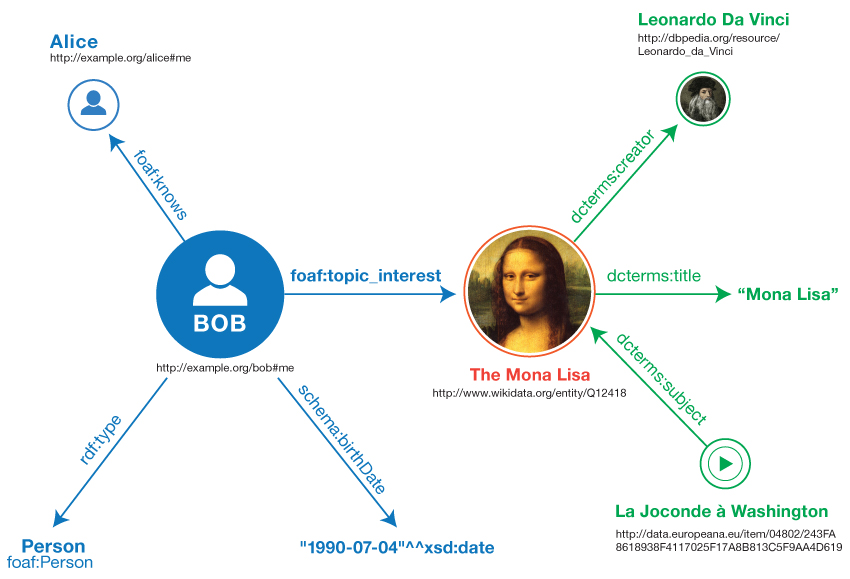
\includegraphics[width=15cm]{rdf-visual-representation-example.jpg}\\
  \caption{Example of RDF Graph}\label{fig:RDFTriple}
\end{figure}

Consider the following Airline Scraper RDF example:
\begin{lstlisting}[language=XML, caption={RDF representation of the flight data}, label={lst:rdf-example}]
  @prefix schema: <https://schema.org/> .
  
  <https://example.com/flights/12345> a schema:Flight;
      schema:departureAirport "Berlin" ;
      schema:arrivalAirport "New York" ;
      schema:airline "Lufthansa" ;
      schema:price "450"^^xsd:decimal ;
      schema:departureTime "10:00 AM"^^xsd:time .
  \end{lstlisting}
  In this scenario scenario, the Airline company has decided to adopt the RDF standard to describe their data.
  Developers can now query the Airline web service without worrying about breaks due to changes in the Airline company \cite{herman2003semanticweb}. 
\\
\\
The RDF standard is not exclusively used by web developers. It is also widely utilized by scientists, engineers, and researchers across various disciplines:
\begin{itemize}
  \item \textbf{Data Scientists}:
  \begin{itemize}
      \item RDF aligns with their work on structured data, semantic queries, and knowledge graphs.
      \item They use RDF to model relationships, extract insights from interconnected datasets, and support machine learning on graph data.
  \end{itemize}
  
  \item \textbf{Computer Scientists and Engineers}:
  \begin{itemize}
      \item They focus on RDF’s theoretical foundations, optimization of storage and querying, and application development for the Semantic Web.
      \item They are often involved in creating RDF tools like RDF stores and query languages.
  \end{itemize}
  
  \item \textbf{Knowledge Engineers}:
  \begin{itemize}
      \item Specialize in designing ontologies and frameworks using RDF to represent knowledge in areas like AI, natural language processing, and expert systems.
  \end{itemize}
\end{itemize}

To assist Scientists in their work, the Semantic Web supports a set of tools and technologies that enable the creation, sharing, and analysis of structured data.
Platforms like Protégé, Apollo, and NeOn are well-known in the ontology engineering community. 

"An Ontology is a knowledge structure used to formally represent and share domain knowledge through the modeling and creation of a framework of relevant concepts and the semantic relationships between the concepts" \cite{ontology}.

These ontology editors offer comprehensive support for creating and editing ontologies and RDF datasets through their graphical user interfaces (GUIs), which enhance visualization and make RDF development easier.

\section{Motivation Scenario\label{sec:moti}}

The following hypothetical scenario illustrates the current situation.
\\
John Doe is a Junior Software Developer and just started working in his first company as Web Developer.
He quickly immersed himself in his daily tasks, working with his favorite IDE, Visual Studio Code, to craft the backbone of their innovative web application—a platform with social media-like features. 
\\
\\
While John primarily worked with VSCode due to its lightweight and customizable nature, he soon realized that his workflow differed significantly from that of his colleagues. Some teammates preferred IntelliJ IDEA for its extensive refactoring tools, while others relied on Protégé because its visual representation of ontologies helped them better understand and manage complex data relationships.
\\
\\
A significant part of the project involved working with RDF files, mainly RDF/XML and Turtle formats, to define the application's semantic data structure and its RDF schema. Although the project repository already contained some instances examples, John found himself losing a lot of time creating a valuable amount of example instances to test the limitation of his RDF schema. This extra step, required to ensure that every modification produced the intended results, often disrupted his coding flow.
\\
\\
Although he is writing in Turtle language for the majority of his time and Turtle is the most readable among all the RDF formats, John also struggles to read and understand many lines of code and often mistake like every other human being. Just like his colleagues, he started using an RDF schema visualizer like "isSemantic.net" or RDF Grapher, to see a graphical representation of his RDF schema \cite{issemantic,rdfGrapher}. The representation helps him a lot to identify relations errors, but importing his schema in another software every time contributes to the interruption of his workflow.


\section{Theses and Scientific Contribution  \label{sec:objective}}
The previous scenario highlights two big challenges. The first is the lack of a seamless integration between specialized development environments and RDF visualization tools. 
Developers should be free to choose the IDE that best suits them, but the disjointed process of visualizing semantic data remains a critical bottleneck.
\\
\\
The second challenge lies in the inefficiency of testing and validating RDF schemas. Manually generating new instances to test schema's limitations remains a major time-consuming task. Developers must invest considerable effort in creating and maintaining test data, moving their focus from core development activities. This repetitive manual work not only delays progress but also increases the risk of inconsistencies and undetected schema flaws.
\\
\\
This Master's Thesis aims to address these challenges and tries to incorporate all developer tools into a single environment.
By developing an IDE extension, developers will be able to handle RDF writing, data visualization, and instance generation in one place.
This IDE extension could support the direct editing of the generated instances, allowing for a more streamlined and efficient workflow.


\section{Positioning within the Scientific Context \label{sec:scope}}
This Thesis is positioned in the domain of Semantic Web and RDFs. It tries to address in the integration of development environments, RDF visualization and RDF instances generation, to enhance both theoretical understanding and practical application in the field.
\\
\\
As stated in the previous sections, the Semantic Web and RDFs, are very important for the scientific community. Their goal is to simplify machines' and computer scientists' lives when extracting and processing a vast amount of information from the W3.
Despite all its advantages, the Semantic Web struggles to move beyond academic use and find widespread commercial applications. 
There is indeed a lack of tools that can help engineers to work with RDFs and the Semantic Web to facilitate the creation and management of RDF Data. 
Among the most popular Integrated Development Environments, like Visual Studio Code, IntelliJ IDEA, and others, we can mainly find extensions that support syntax highlighting, with grammar checker and SHACL validators, and only one VSCode extension for the visualization of RDFs limited to the N3 and Turtle formats \cite{vscode_rdf_plugin,jetbrains_rdf_plugin,stackoverflow_survey_2024} (see Figure~\ref{fig:RDF-term-in-vscode-marketplace}).
\begin{figure}[htb]
  \centering
  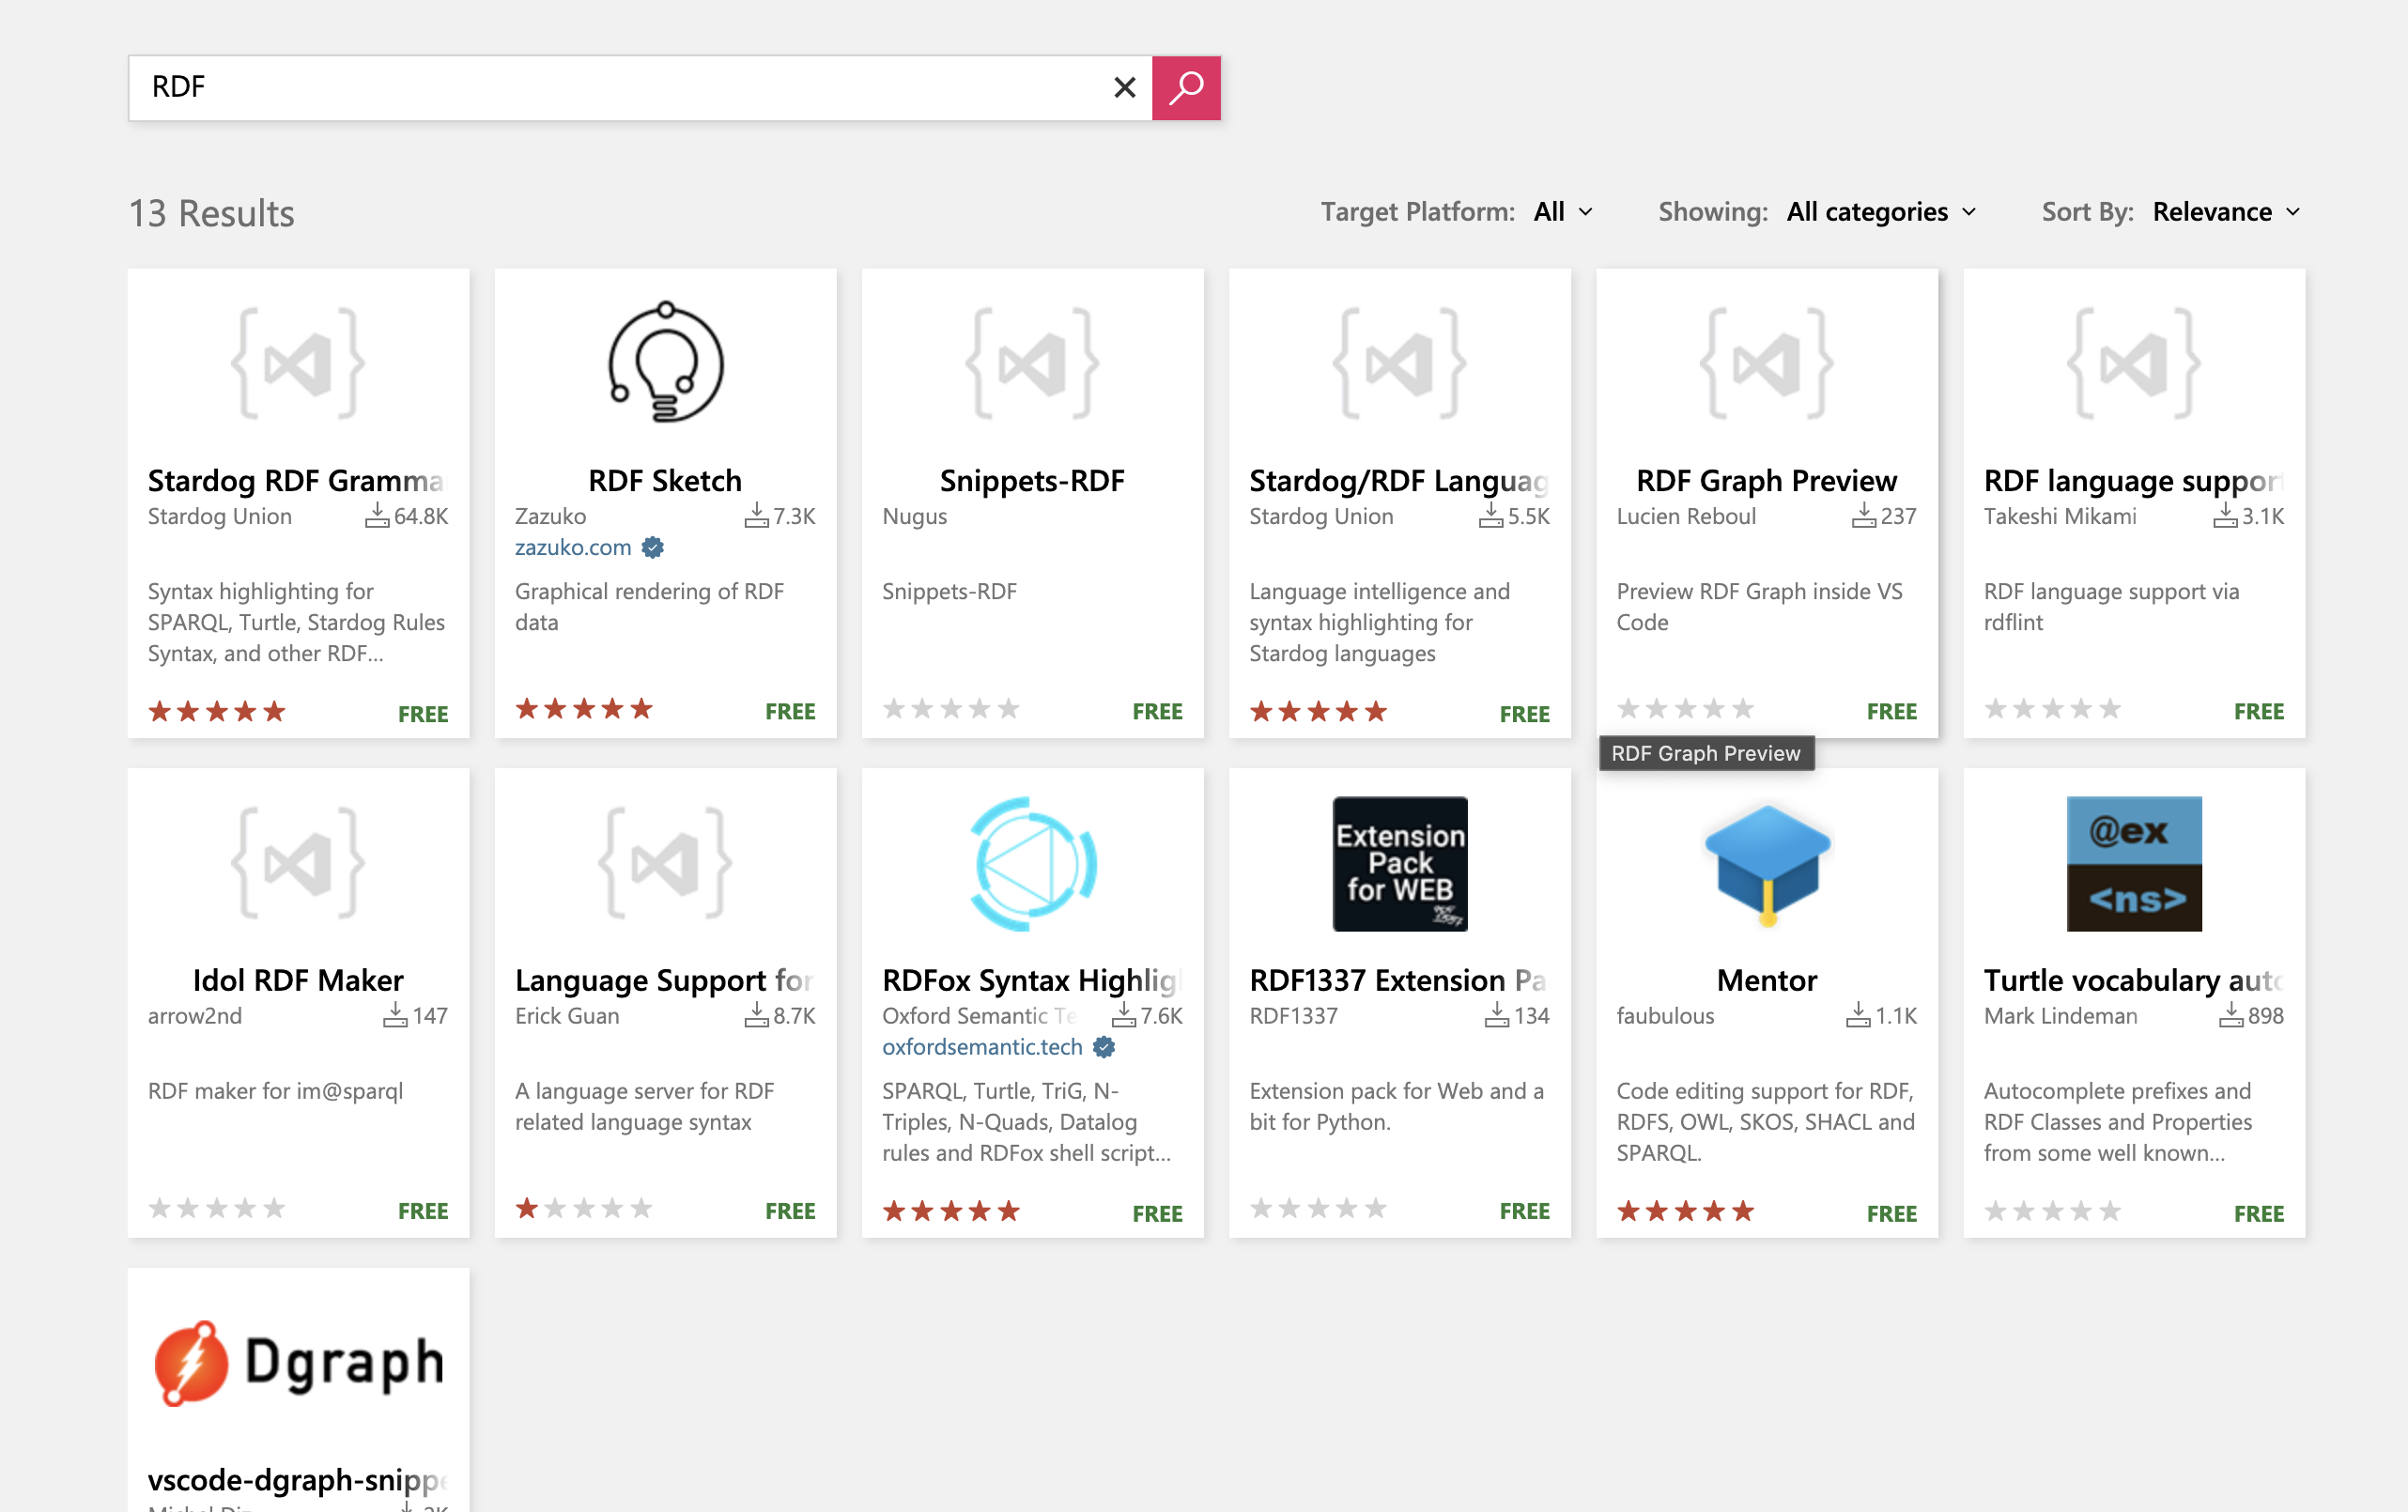
\includegraphics[width=13cm]{RDF-term-in-vscode-marketplace.png}\\
  \caption{Limited Support: A Search for 'RDF' in the Plugin Marketplace Yields Only 13 Results, Highlighting the Scarcity of RDF-Specific Extensions for Developers.}\label{fig:RDF-term-in-vscode-marketplace}
\end{figure}
\\
\\
The Semantic Web community needs a solution that could bridge this gap, something that is not limited to a specific software, architecture, or environment. A solution that could potentially be compatible with every IDE and Browser. An open-source software with and MIT license can be enhanced not just by the community, but also by companies and institutions.
A program with a core that allows an easy integration of modules and plugins. 
\\
\\
For this Master's Thesis, I will develop a Web Service using Python 3.11 and the Fastapi library, able to process the most common RDF formats, generate n amount of instances for a given RDF Schema, and return the desired results. 
The outcome will be provided in different formats, but mainly served as HTML pages, so that can be processed by a Visual Studio Code extension in a Web View. This approach will limit the service to be used only by the VSCode IDE, but by all the ones that support rendering of HTML content in their environment.
\\
\\
To prove the validity of this approach, I will develop not just the Visual Studio Code extension using TypeScript, but also a dedicated browser frontend view, and an IntelliJ IDEA plug-in, in Kotlin, with a limited set of features. 
These Client Side applications will communicate with the Web Service, and via REST calls. The user will be able to: 
\begin{itemize}
      \item Send an RDF Schema to the Web Service
      \item Request an n amount of instances for the given schema
      \item Edit the RDF Schema with the instances generated by the server
      \item Visualize the RDF
      \item Download the Graph as an image. 
\end{itemize}
% limitations
Due to the vastness of this project, some features will only be deepened in a theoretical manner, like the AI Instance Generation, and only some because features for the IntelliJ IDEA plugin will be covered.
\\
\begin{figure}[htb]
  \centering
  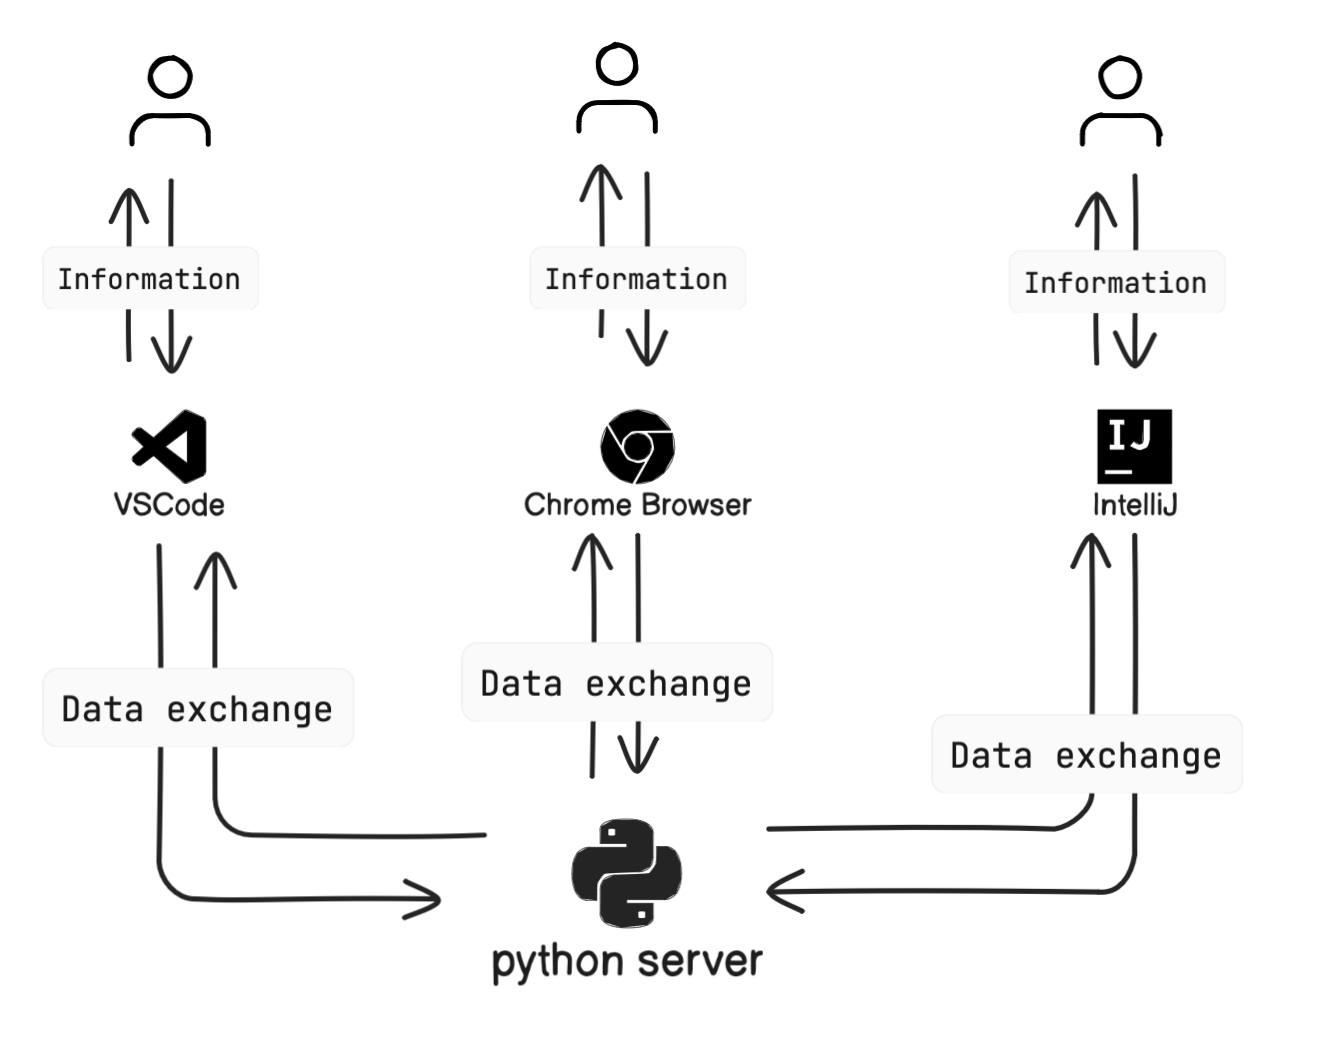
\includegraphics[width=13cm]{schema_architecture_1_white.png}\\
  \caption{System Architecture: Information Flow and Data Exchange between Users, Development Environments (VSCode, IntelliJ), Chrome Browser, and a Python Server.}\label{fig:intro}
\end{figure}

\section{Structure of the Work \label{sec:outline}}

This thesis is separated into 7 chapters.
\\
\\
\textbf{Chapter \ref{cha:chapter2}: State of the Art} covers the related work in the RDF world, from the instance generation to the graph visualization. 
\\
A short view of existing tools and projects in the same domain, like GAIA and Ontodia.
\\
A comparison of the two different approaches in terms of instance creation (Manual vs Automatic).
% in this actually you should talk a lot about A-BOX and T-Box
A brief look at the current standards and technologies compatible with the semantic Web and RDFs.
\\
\\
\textbf{Chapter \ref{cha:chapter3}: Concept} includes the requirements for the project, a view of the technologies and high-level architecture, and the constraints and goals of this work.
\\
\\
\textbf{Chapter \ref{cha:chapter4}: Implementation} features the implementation of the project with all its components. Describe in very detail the design choices, building blocks, and algorithms of this system.
\\
\\
\textbf{Chapter \ref{cha:chapter5}: Evaluation} explains how the implementation is validated. Portrays benchmarks and measurements regarding the performance of the solution. Showcases some examples of RDF generation and graph visualization. Cite the experience of a group of Computer Scientists. 
\\
\\
\textbf{Chapter \ref{cha:chapter6}: Conclusion and Limitations} summarizes the thesis, describes the problems that occurred. 
\\
\\
\textbf{Chapter \ref{cha:chapter7}: Outlook} Discusses the future of the project, and the possible improvements that can be done, like the integration of an AI model and the support for further ontologies.
    \chapter{State of the Art\label{cha:chapter2}}

This chapter is intended to give an introduction about relevant terms, technologies and standards in the field of Semantic Web. It also delves into similar and related implementations (i.e. GAIA) to provide a comprehensive understanding of the current state of the art.

\section{Technologies \label{sec:tech}}

This section covers the fundamental technologies, specifically RDF and SPARQL, which serve as the foundational building blocks for structuring and querying data.

\subsection{RDF (Resource Description Framework)\label{sec:rdf_primer}}

The RDF is the foundation of the Semantic Web. It's a framework for describing resources on the Web thanks to URIs. A resource could be anything: a human being, a document, an object a concept \cite{rdf}. 
\\
\\
Specifically, RDF can be used to share and interlinked data. For example, if the following URI \space \textbf{http://www.example.org/bob\#me} is retrieved, it can provide information about Bob, such as his name, his age, and his friend.
If his friends' International Resource Identifiers (IRIs) are retrieved, like Alice's, more information regarding them can be accessed (i.e. more friends, interests, etc.). This process of "link navigation" is called Linked Data \cite{rdf}.
\\
\\
This RDF property can be useful for many use cases like: 
\begin{itemize}
	\item Creating distributed social networks by interlinking RDF descriptions of users.
	\item Integrating API feeds to ensure seamless discovery of additional data and resources by clients.
	\item Embedding machine-readable data into web pages.
	\item Standardizing data exchange across databases.
\end{itemize}

RDF interlinks resource with "statements". A statement is a triple containing a subject, a predicate, and an object.
The subject and the object stand for the resources that need to be represented. The predicate is the type of relation between those resources, and it is always phrased in one directional way (from the subject to the object). 
\\
This relation between the two is called a Property \cite{rdf}.
\\
It is possible to visualize these Triples as Graphs (see Figure \ref{fig:RDFTriple}) and query them using SPARQL.
\\
\\
In an RDF file, three type of data can  occur :IRIs, literals and blank nodes. 
\begin{itemize}
	\item IRIs are the identifiers of the resources. They are similar to the Uniform Resource Locators (URLs), but they don't provide information about where the resource is located or how to access it. They can only be used as mere identifiers. IRIs can appear in all three positions of a triple. 
	\item Literals are all the values that are not IRIs. They can be strings, numbers, dates, etc. They can only appear in the object position of a triple.
	\item Blank Nodes are all the nodes of a graph that are not identified by an IRI. They are like simple variables in algebra that represent something without saying what their value is. Blank nodes appear in the subject and object position of a triple. 
\end{itemize}
RDF allows grouping multiple RDF statements into multiple graphs and associate them with a single URI. 

\begin{lstlisting}[language=XML, caption={RDF Grouped Data}, label={lst:xml-rdf-grouped-example}, frame=single]
	<Bob> <is a> <person>.
	<Bob> <is a friend of> <Alice>.
	<Bob> <is born on> <the 4th of July 1990>.
	<Bob> <is interested in> <the Mona Lisa>.
\end{lstlisting}
One of the related problems with RDF is that the data model doesn't make assumptions about what resource URIs stand for.
For example the statement \space \textbf{ex:Apple ex:isLocated ex:California}, without any additional information about Apple, could be misleading. Without additional context Apple could refer to a fruit in California or Apple incorporated in Cupertino.
\\
One solution to this problem is to use IRIs in combinations with Vocabularies and other conventions that add semantic information about the resources.
\\
\\
In order to include Vocabularies in an RDF graph, RDF provides a Schema language.
\\
The RDF Schema allows the description of groups of related resources and the relations between them.
The class and property system is close to an object-oriented programming language. The difference with this model is that the RDF schema defines the properties in terms of Class and not vice versa as in object-oriented programming.
\begin{table}[h]
    \centering
    \begin{tabular}{lll}
        \toprule
        \textbf{Construct} & \textbf{Syntactic form} \\
        \midrule
        Class (a class) & C \texttt{rdf:type rdfs:Class}  \\
        Property (a class) & P \texttt{rdf:type rdf:Property} \\
        type (a property) & I \texttt{rdf:type C} \\
        subClassOf (a property) & C1 \texttt{rdfs:subClassOf C2} \\
        subPropertyOf (a property) & P1 \texttt{rdfs:subPropertyOf P2} \\
        domain (a property) & P \texttt{rdfs:domain C} \\
        range (a property) & P \texttt{rdfs:range C} \\
        \bottomrule
    \end{tabular}
    \caption{RDF Schema Constructs}
    \label{tab:rdf_schema_constructs}
\end{table}

An RDF Class is a group of resource with common characteristics. The resources in a class are referred to as instances of that class.
\\
\\
As discussed in previously, properties are used to describe the relations between subject and object resources.
The main properties for the construct of RDF schema are: 
\begin{itemize}
	\item \textbf{subClassOf} is used to state that all the instances of one class are instance of another.
	\item \textbf{subPropertyOf} is used to define that all resources related by one property are also related by another.
	\item \textbf{domain} is used to declare to which domain / class that property belong to.
	\item \textbf{range} is used to indicate the type of the property value.
\end{itemize}

RDF supports 4 main types of formats: The "Turtle family of RDFs", JSON-LD, RDF/XML and RDFa \cite{rdf}.


%  fix the citations.

\subsection{SPARQL \label{sec:bbb}}
In the RDF world, there are 2 main ways to retrieve data from an RDF store. The first one is to simple is to use a REST Endpoint and perform CRUD operations on the DB. This is in many cases the quickest solution, because it doesn't required new knowledge or new knowhow. 
The main problem is when the RDF store doesn't allow HTTP CRUD or doesn't provide a REST Endpoint.
In these cases the second solution is to use SPARQL.
\\
\\
SPARQL is a set of specifications that provide tools to retrieve and manipulate RDF graph content on the W3 or in an RDF store.
One of this tool is the SPARQL Query Language \cite{sparql}.
\\
\\
The SPARQL Query Language it's a query language, not far from the most well known SQL, is used for query formulation and retrieval of on the web.
\begin{lstlisting}[language=SPARQL, caption={Example of SPARQL Query}, basicstyle=\ttfamily, frame=single]
    PREFIX foaf: <http://xmlns.com/foaf/0.1/>
    SELECT ?name (COUNT(?friend) AS ?count)
    WHERE { 
        ?person foaf:name ?name . 
        ?person foaf:knows ?friend . 
    } GROUP BY ?person ?name
\end{lstlisting}

In order to make the exchange of query results among machines, SPARQL supports the following exchange formats: XML, JSON, CSV and TSV \cite{sparql}.



\section{Related Work \label{sec:tech}}

This section provides a detailed overview and analysis of the related work.

\subsection{GAIA (Automatic Instance Generator for Abox)}

The GAIA project, is a RDF triple generation tool developed by CEDAR. 
This research introduces an OWL-based generic RDF triple generator capable of loading any OWL ontology schema and generating compliant RDF instances, unlike the LUBM instance generator, which only supports its predefined LUBM ontology.
It strictly relies on OWL because the majority of ontologies that are currently available are written using this language \cite{raynaud2014gaia}.
\\
\\
GAIA is designed for performance and scalability, thanks to the multithreading implementation that allows to generate a large volume of triples, making it perfect for ontology benchmarking or synthetic dataset generation \cite{raynaud2014gaia}.
\\
\\
Despite its performance and accuracy, GAIA has several limitations. The software is missing a schema visualization system or interactive graph explorer. This makes it hard for a human to visualize at glance the newly generated instances.
The system is also not limited to machines with JAVA installed on it, and having it implemented as IDE extension is a very challenging task due to its architecture.
\\
Furthermore, GAIA does not natively support RDF Schema (RDFS) or lightweight RDF graphs in Turtle or JSON-LD format (it only supports $.RDF$ or $.XML$).

\begin{lstlisting}[language=XML, caption={Example of RDF/XML Data}, basicstyle=\ttfamily\footnotesize, frame=single]
    <?xml version="1.0" encoding="UTF-8"?>
    <rdf:RDF xmlns:rdf="http://www.w3.org/1999/02/22-rdf-syntax-ns#"
             xmlns:owl="http://www.w3.org/2002/07/owl#"
             xmlns:rdfs="http://www.w3.org/2000/01/rdf-schema#"
             xmlns:ex="http://example.org/"
             xml:base="http://example.org/ontology"
             xmlns:xsd="http://www.w3.org/2001/XMLSchema#">

        <owl:Ontology rdf:about="http://example.org/ontology">
            <owl:versionInfo>1.0</owl:versionInfo>
        </owl:Ontology>

        <rdf:Description rdf:about="http://example.org/Class/Person">
            <rdf:type rdf:resource="http://www.w3.org/2002/07/owl#Class"/>
            <rdfs:label>Person</rdfs:label>
        </rdf:Description>

        <rdf:Description rdf:about="http://example.org/Class/Organization">
            <rdf:type rdf:resource="http://www.w3.org/2002/07/owl#Class"/>
            <rdfs:label>Organization</rdfs:label>
        </rdf:Description>

        <rdf:Description rdf:about="http://example.org/Individual/JohnDoe">
            <rdf:type rdf:resource="http://example.org/Class/Person"/>
            <ex:name>John Doe</ex:name>
        </rdf:Description>

        <rdf:Description rdf:about="http://example.org/Individual/AcmeCorp">
            <rdf:type rdf:resource="http://example.org/Class/Organization"/>
            <ex:name>Acme Corporation</ex:name>
        </rdf:Description>

    </rdf:RDF>
\end{lstlisting}

\begin{figure}[H]
    \centering
    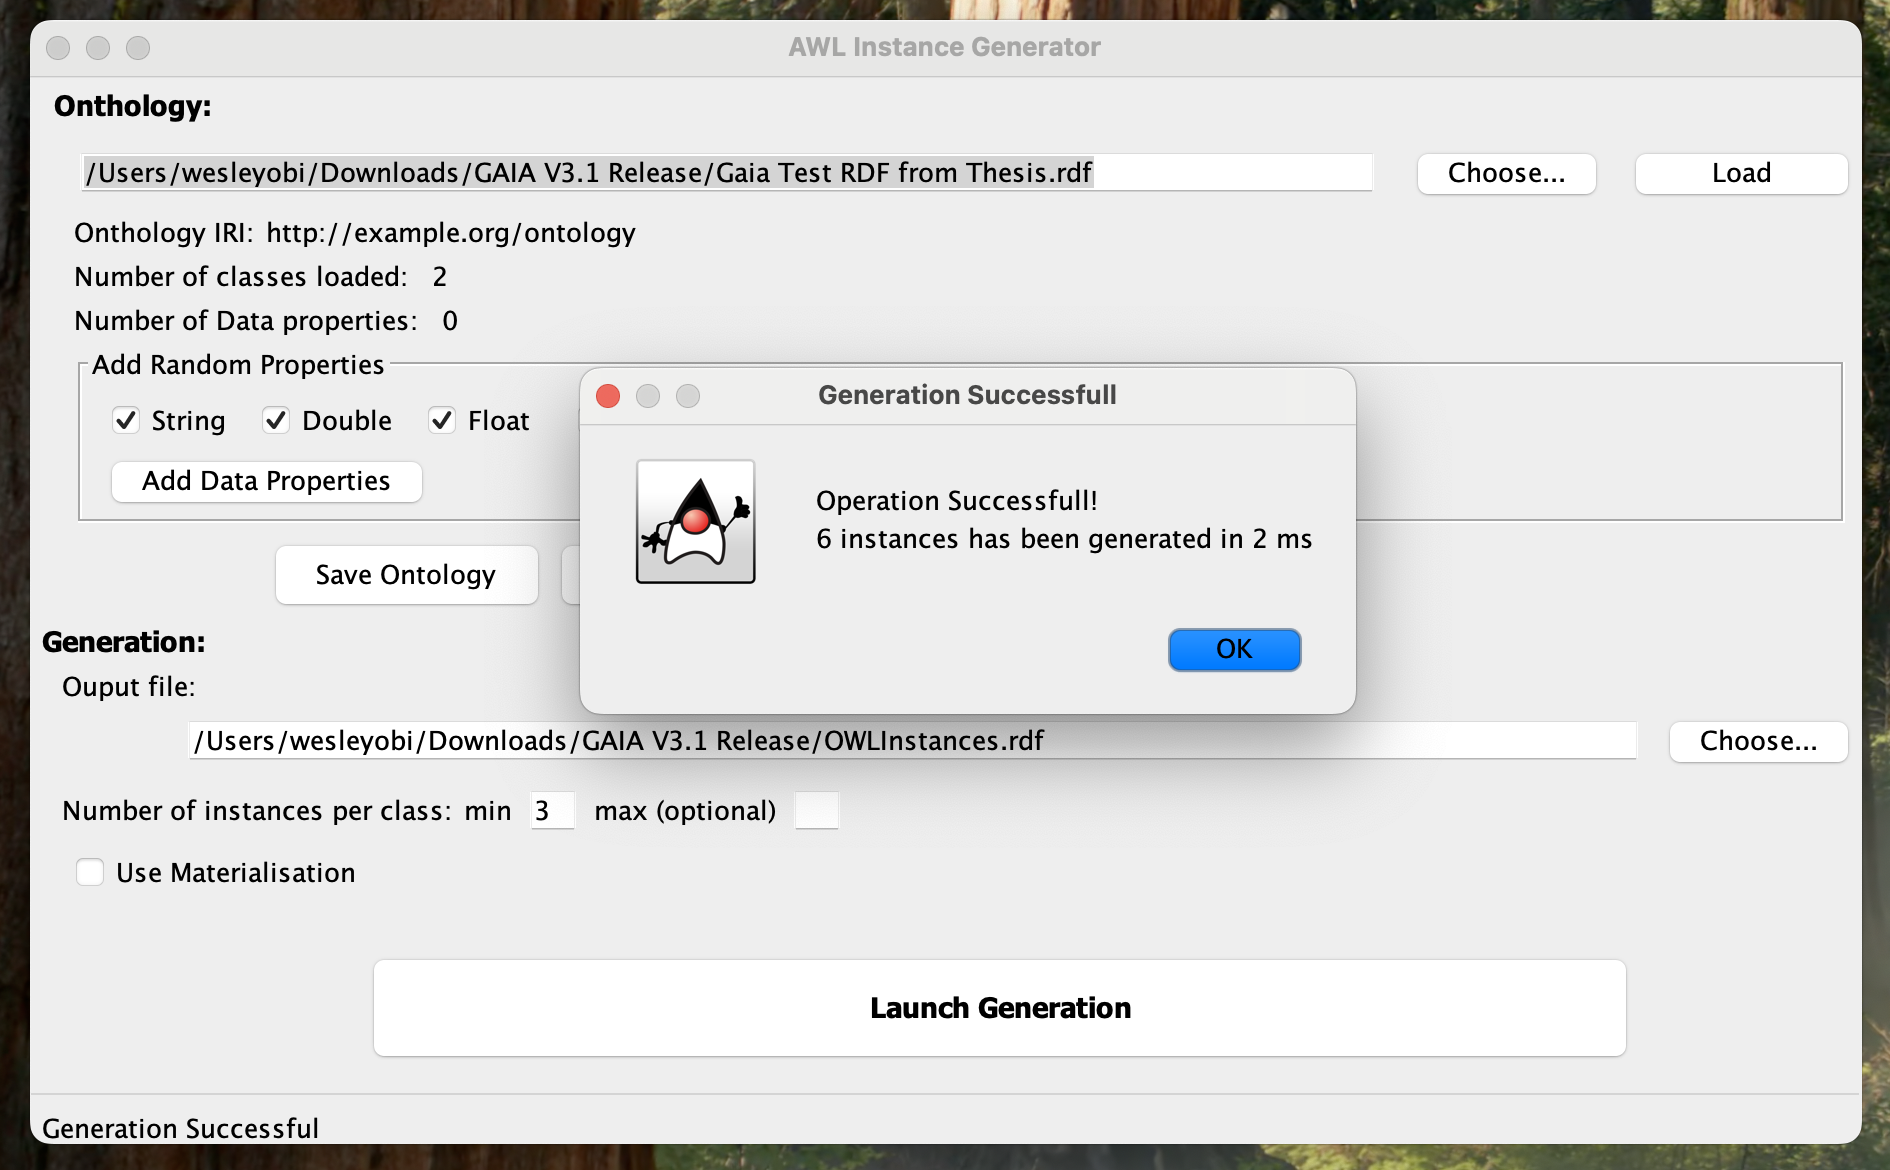
\includegraphics[width=13cm]{GAIA.png}\\
    \caption{GAIA Instance Generator used via GUI}\label{fig:gaia}
  \end{figure}

  \begin{lstlisting}[language=XML, caption={Results of RDF/XML generated instances}, basicstyle=\ttfamily\footnotesize, frame=single]
    ...
    <!-- Instances Generated by OWL_GENERATOR -->

    <owl:NamedIndividual rdf:about="http://example.org/ontology#Organization_instance0">
        <rdf:type rdf:resource="http://example.org/ontology#Organization"/>
    </owl:NamedIndividual>

    <owl:NamedIndividual rdf:about="http://example.org/ontology#Organization_instance1">
        <rdf:type rdf:resource="http://example.org/ontology#Organization"/>
    </owl:NamedIndividual>

    <owl:NamedIndividual rdf:about="http://example.org/ontology#Organization_instance2">
        <rdf:type rdf:resource="http://example.org/ontology#Organization"/>
    </owl:NamedIndividual>

    <owl:NamedIndividual rdf:about="http://example.org/ontology#Person_instance0">
        <rdf:type rdf:resource="http://example.org/ontology#Person"/>
    </owl:NamedIndividual>

    <owl:NamedIndividual rdf:about="http://example.org/ontology#Person_instance1">
        <rdf:type rdf:resource="http://example.org/ontology#Person"/>
    </owl:NamedIndividual>

    <owl:NamedIndividual rdf:about="http://example.org/ontology#Person_instance2">
        <rdf:type rdf:resource="http://example.org/ontology#Person"/>
    </owl:NamedIndividual>

    </rdf:RDF>
\end{lstlisting}

\subsection{The instance Generator project suggested by the professor}
...

\subsection{RDF Graph Preview}

The Graph RDF Graph Preview it's an open source project developed by Lucien Reboul \cite{rdfpreview2022}.
\\
It's a VSCode extension that allows to load RDF files and visualize them as graphs. It uses the D3.js library as core graph rendering system.
\\
\\
One advantage of this extension is that it allows to quickly visualize RDF graph without leaving the current workspace. 
\\
But unfortunately, this plugin is only able to render RDF files written Turtle and N-Triples/N3 formats. The tool provides no support for automatic instance generation, forcing users to do all the heavy work manually.
\\
\\
\begin{figure}[htb]
    \centering
    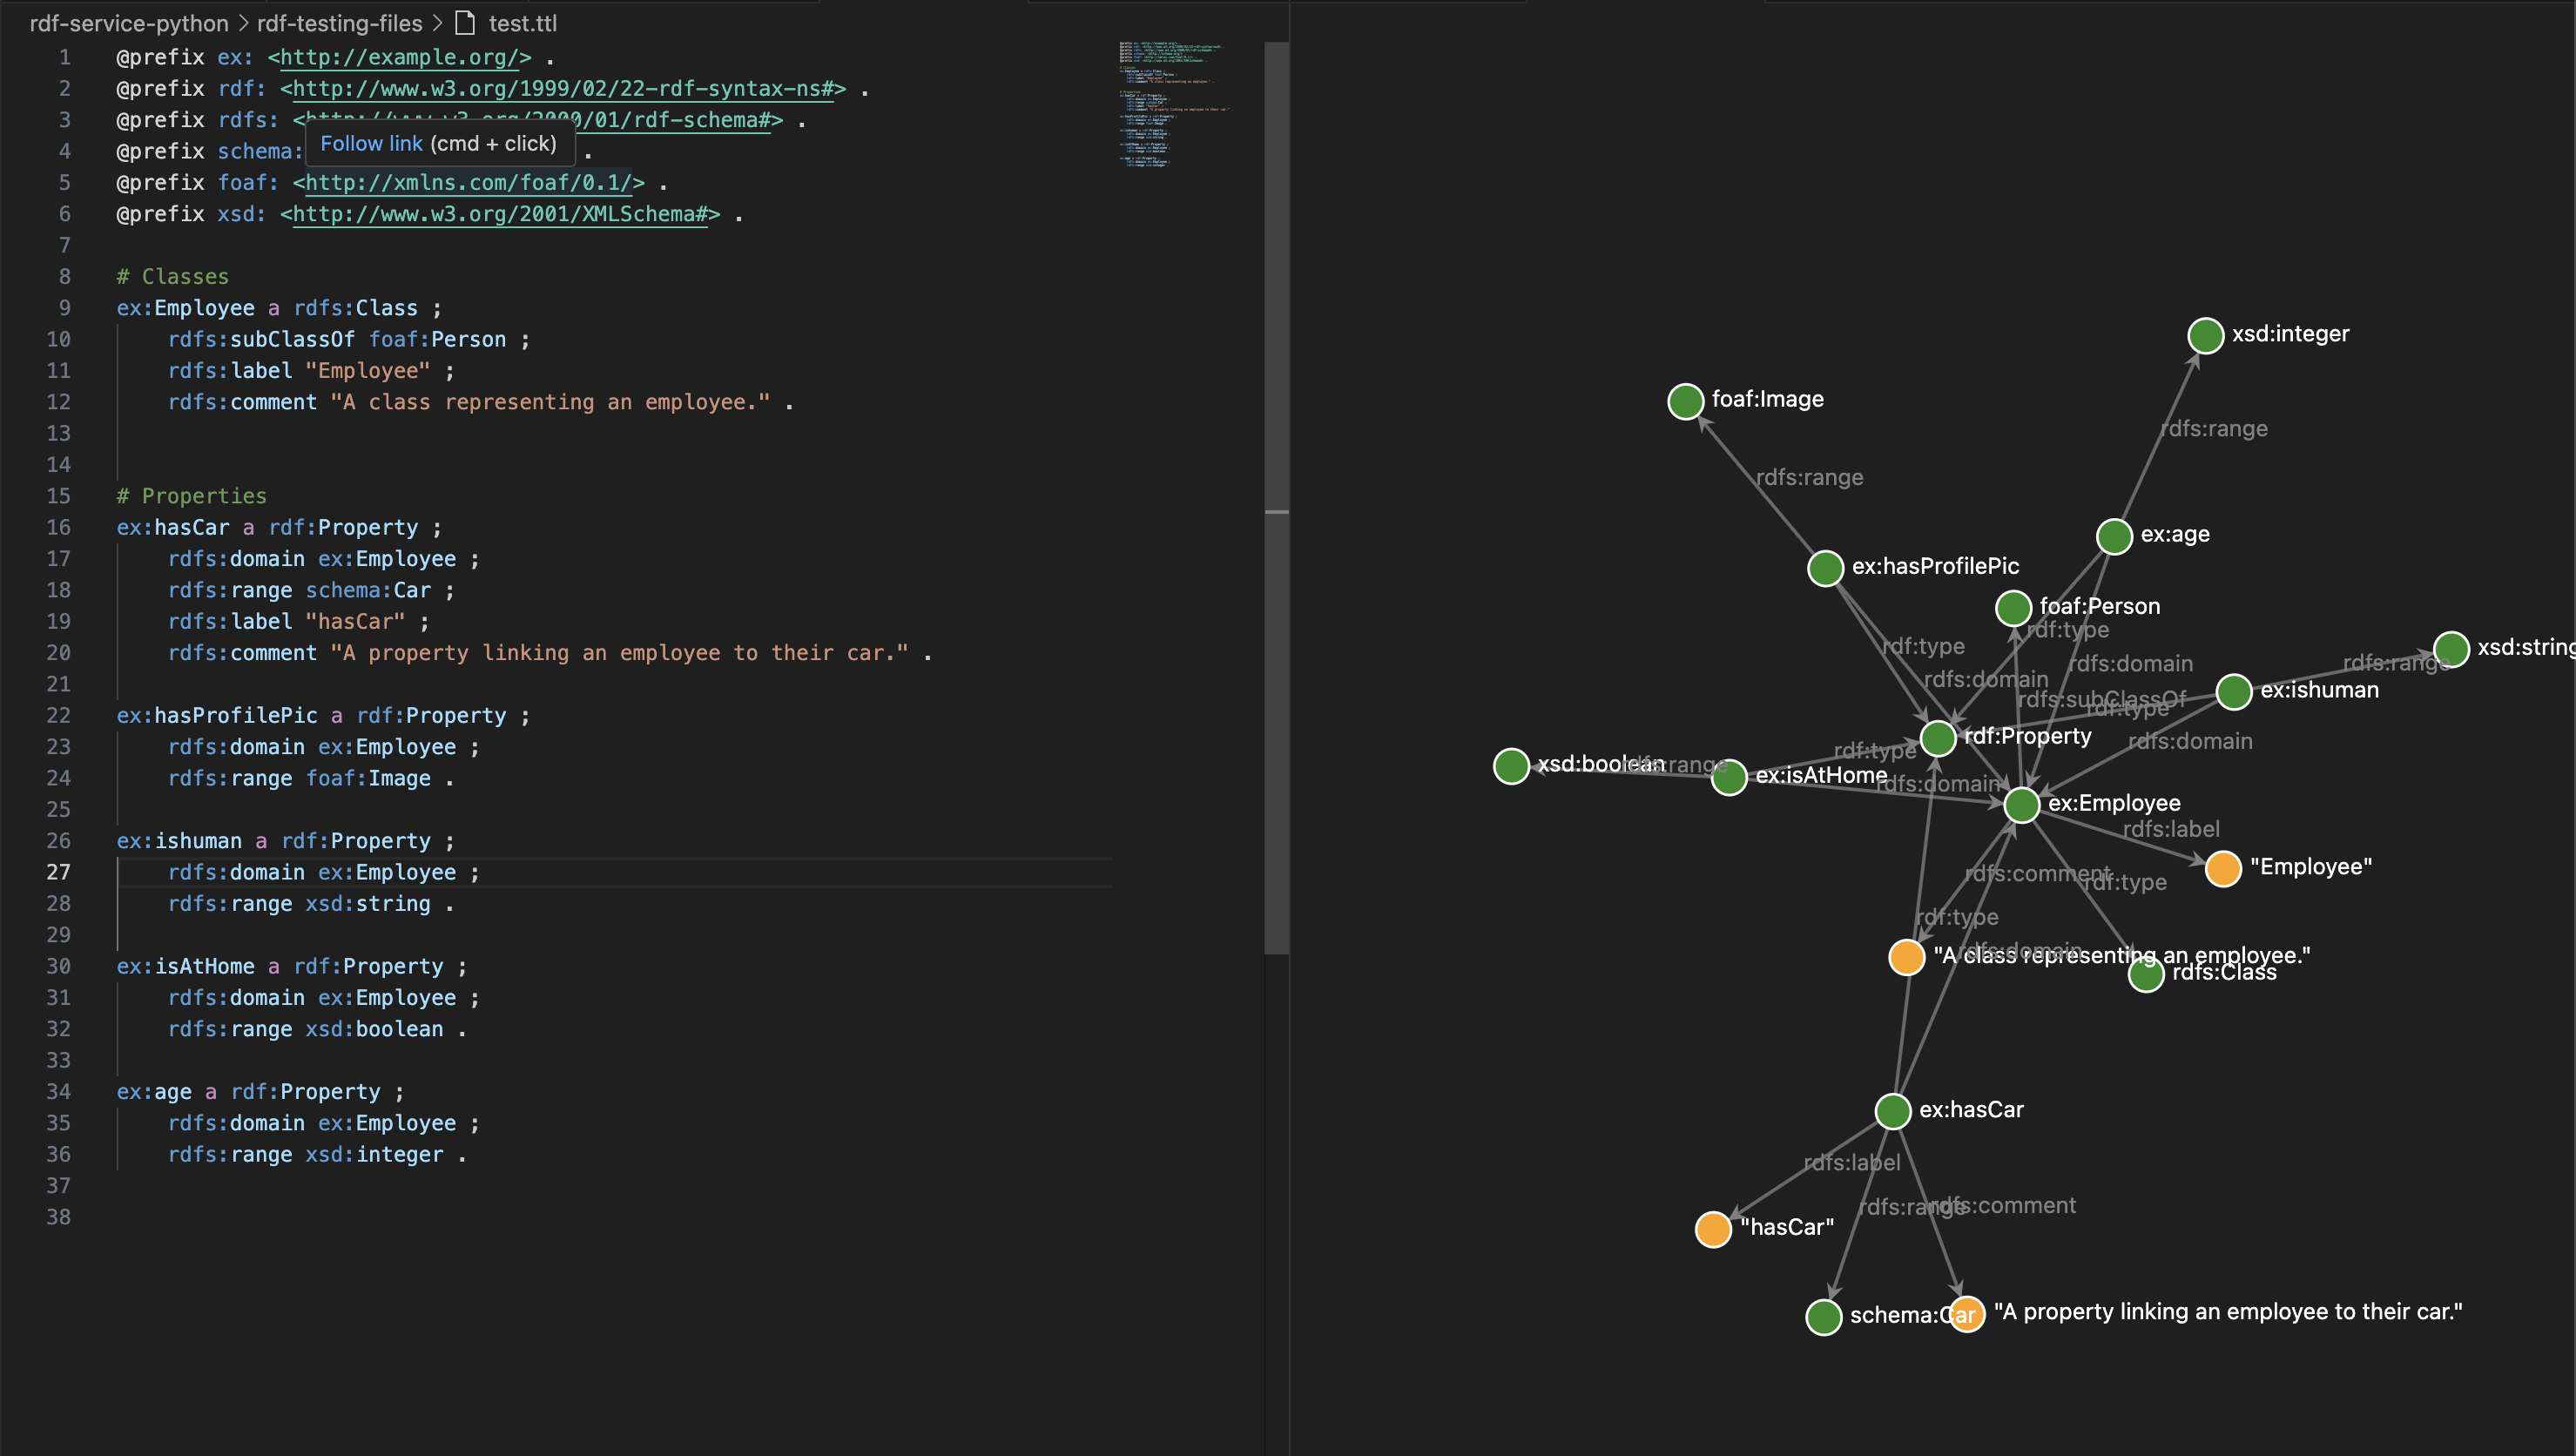
\includegraphics[width=13cm]{RDFPreviewExtension.png}\\
    \caption{RDF Graph Preview VSCode Extension}\label{fig:RDFPreviewExtension}
  \end{figure}
  

% write about  another RDF instance generation project,
% the ontodia maybe? 
% also protégé 
    \chapter{Consept\label{cha:chapter3}}
This section determines the requirements and design choices necessary for developing the RDF Instance Generator Schema Visualizer and the RDF web service.

\section{Overview\label{sec:reqoverview}}

This project aims to simplify RDF schema exploration, validation, and instance generation. To achieve this the following requirements are defined: 
\begin{itemize}
    \item Functional requirements, for core features like, instance generation, schema validation, and visualization.
    \item Non-functional requirements, to take into account performance, usability and compatibility.
    \item Technical requirements, specified for underlying technologies and system design.
    \item Data privacy and Security, useful to ensure the security and privacy of user data.
\end{itemize}

The design prioritizes a client-server architecture, and cross-platform compatibility to enhance usability and efficiency. 
\\
The Web Service is designed to be compatible with various Browsers and IDEs. 
\\
The IDE extension will support users and will seamlessly integrate in their workflow.
\section{Functional requirements\label{sec:techreq}}
In this section covers the functional requirements for the entire system.

\subsection{Instance Generation\label{sec:reqsuba}}
The very first requirement for this project is the generation of synthetic RDF instances.
\\
When the user is writing an RDF file, in turtle, N3, XML or other RDF formats, it will generate some synthetic RDF instances that could save him a lot of time avoiding the insertion of testing data.
\\
The application will not just generate compatible triples instances, but also allow the user to modify the automatically generated instances.

\subsection{Schema Validation\label{sec:reqsuba}}
The Program should be designed to validate a user-defined RDF schema by checking the structural integrity and semantic consistency of its triples. 
Each triple conforms to syntactic constraints (e.g., proper use of IRIs, literals, and blank nodes) and the asserted relationships lead to any logical contradictions or unexpected inferences.
\\
In case of errors in the schema description, feedback should be provided to the user, via UI or Terminal.

\subsection{Multi-Vocabulary Support\label{sec:reqsuba}}
Interoperability and semantic richness are crucial for ensuring seamless data integration, enhancing knowledge representation, and enabling efficient querying and reasoning across diverse RDF datasets.
By supporting multiple vocabularies and ontologies such as RDFS, FOAF, Schema.org and others, the system should be able to handle a wide range of RDF data sources and their visualization as graphs.

\subsection{Import and Export\label{sec:reqsuba}}
The software should allow the users to import their custom RDF files, and export the file with the automatic generated instances in the same format.

\subsection{Schema Visualization\label{sec:reqsuba}}
To simplify the exploration and analyzes of an RDF from a human eye, the program should be able to display the described RDF schema with its graphical representation.
The displayed graph should have some interactive features like zooming, panning and node collapse.
\\
The graphical representation should adapt based on the schema complexity and hierarchical structure.
\\
In the IDE  extension, the user should be able to visualize the graph in a side panel window next to the RDF file their working on. 

\section{Non-functional requirements\label{sec:techreq}}
This section determines the non-functional requirements of the system.

\subsection{Performance\label{sec:reqsuba}}
The system should ensure high performance rendering of large RDF graphs to facilitate seamless visualization and interaction. Additionally, operations such as node selection and zooming should be executed with minimal latency to maintain a responsive user experience. The system should optimize rendering pipelines to support real-time exploration of complex RDF schemas without compromising efficiency.

\subsection{Usability\label{sec:reqsuba}}
Both the IDE extension and the web application should feature an intuitive and user-centric interface that enhances accessibility and minimizes the learning curve for users. To achieve this objective, the design should incorporate familiar UI elements or skeuomorphic design principles, ensuring a seamless and intuitive user experience. 

\subsection{Compatibility\label{sec:reqsuba}}
To ensure seamless integration across various development environments, the web service should be designed with cross-platform compatibility, enabling effortless adoption in different IDEs with minimal modifications. This approach enhances interoperability, allowing the service to function efficiently within diverse software ecosystems while maintaining consistent performance and usability. 
\\
To validate this, minor features in a secondary IDE should be implemented.


\section{Technical Requirements\label{sec:techreq}}

\subsection{Web Architecture\label{sec:reqsuba}}
The system should be designed with a client-server architecture. There are no constraints on the specific technologies (e.g. SOAP, REST, gRPC), but it must follow the web principles and use Web technologies, such as HTML, CSS, JavaScript or WebAssembly, and protocols (e.g. HTTP, WebSockets).

\subsection{IDE extension\label{sec:reqsuba}}
The application should be accessible via a web-based client to ensure broad availability; however, primary emphasis should be placed on its integration as an extension within widely used IDEs. 

\section{Data privacy and Security\label{sec:techreq}}
\subsection{Security\label{sec:reqsuba}}
To ensure the confidentiality and integrity of RDF data, the system should implement secure data transmission protocols, such as HTTPS, to protect sensitive information during transmission.

\subsection{Confidentiality\label{sec:reqsuba}}
Based on the current design, no information should be saved from the Business Logic Layer. 
\\
All data processing occurs in-memory, either on the client-side or server-side, ensuring that no persistent storage of user data takes place within the system. This ephemeral data handling approach significantly reduces the risk of data retention and unauthorized access. As a result, compliance requirements related to long-term data storage, such as those outlined in the General Data Protection Regulation (GDPR), are minimized. 


\section{Solution strategy\label{sec:techreq}}
As stated previously in the requirements section, the system is designed with a client-server architecture, where the client and server play distinct roles in the overall functionality.

\begin{figure}[H]
    \centering
    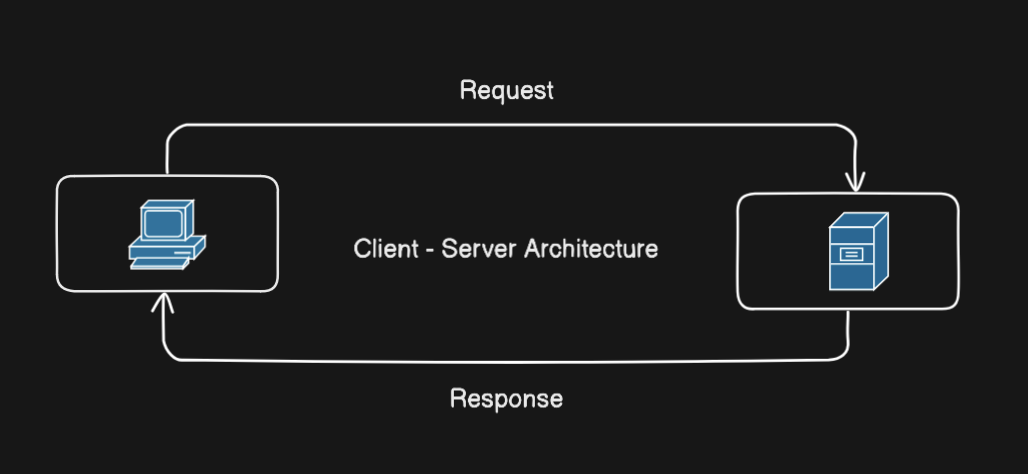
\includegraphics[width=14cm]{client_server.png}\\
    \caption{Client / Server}\label{fig:client_server}
  \end{figure}

\subsection{Client\label{sec:reqsuba}}
To ensure a broad availability of the system, the system is designed to support two type of user-agents:
\begin{itemize}
    \item Browsers
    \item Integrated Development Environments 
\end{itemize}
The Browser chosen by the user, should be able to access the web application via HTTP requests protocol.
The user will then upload their RDF file and send it to the server.
The Client will then receive the processed information and display the resulting graph (see Figure \ref{fig:BrowserGraphView}).

\begin{figure}[htb]
    \centering
    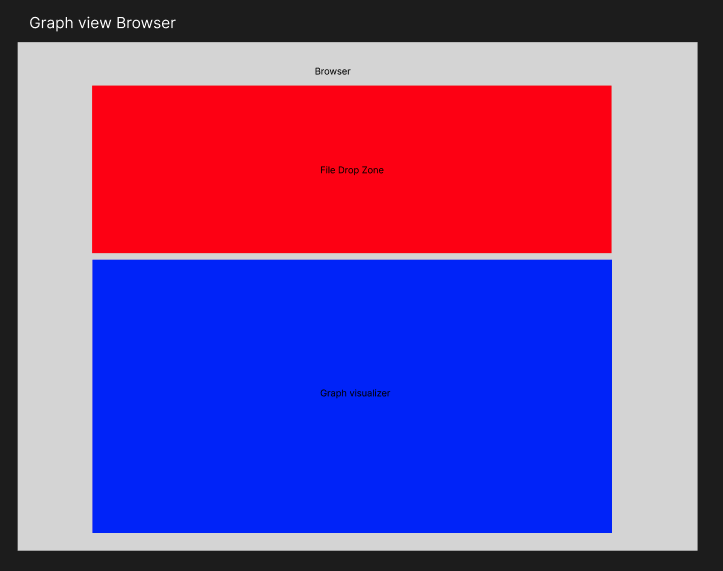
\includegraphics[width=14cm]{mock dropzone.png}\\
    \caption{Browser file drop zone and graph view }\label{fig:BrowserGraphView}
  \end{figure}

In addition to this, the user should be able to read the RDF file with the generated instances next to its graphical representation (see Figure \ref{fig:BrowserRDFReader}).

\begin{figure}[htb]
    \centering
    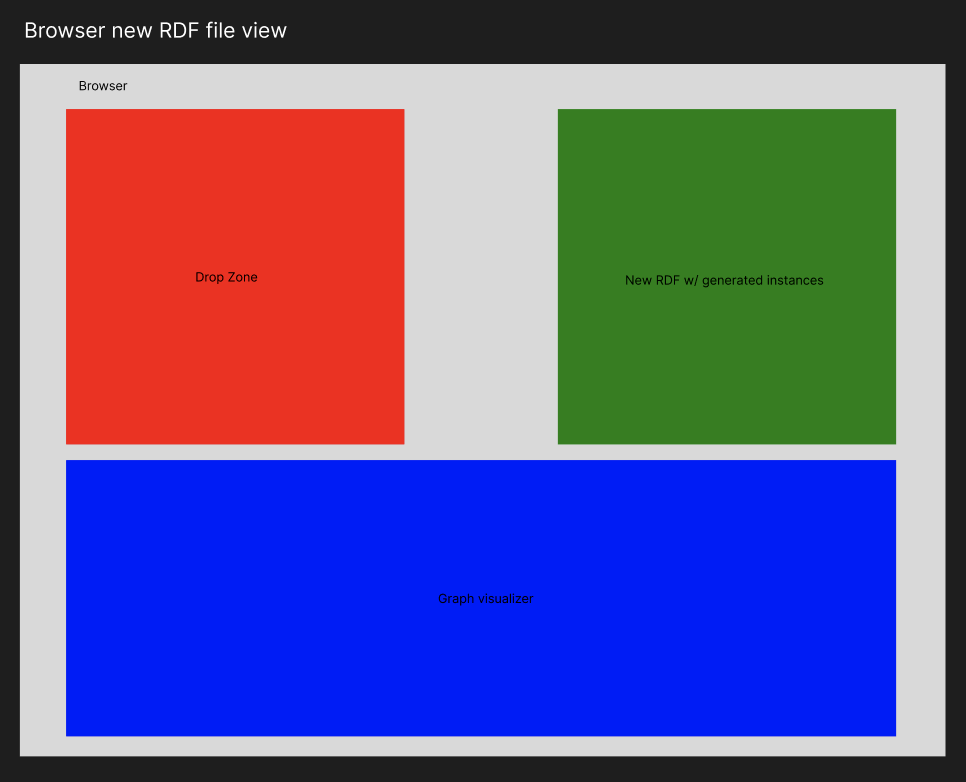
\includegraphics[width=14cm]{mock_browser_new_RDF_instance.png}\\
    \caption{Browser new RDF side panel view }\label{fig:BrowserRDFReader}
  \end{figure}

Within the IDE, the user experience UX will be slight different from the Browser one. Instead of manually uploading an RDF file, users will interact with the system directly within the IDE. By working on an RDF file and executing a predefined command, a web-based visualization panel of the file on focus will be dynamically launched as a side panel within the IDE. This panel will render an interactive graphical representation of the RDF schema in real time, allowing users to analyze relationships, structures, and dependencies without disrupting their coding environment (see Figure \ref{fig:IDEGraphView}). 

\begin{figure}[H]
    \centering
    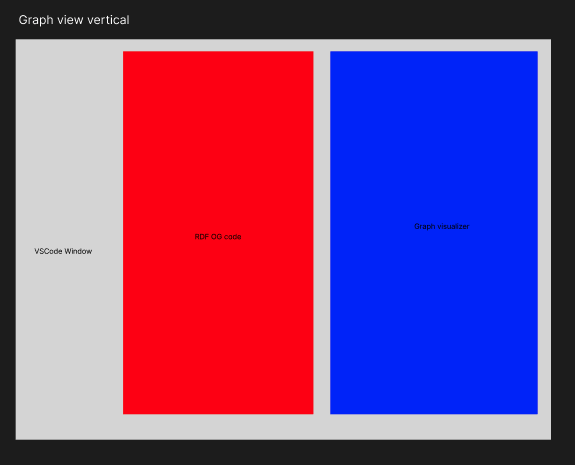
\includegraphics[width=14cm]{mockup side panel view.png}\\
    \caption{IDE Graph side panel view}\label{fig:IDEGraphView}
  \end{figure}

  The extension will not only support the visualization of RDF files in the format requested by the user, similar to its browser counterpart, but it will also enable real-time modification of the file (see Figure \ref{fig:IDERDFReader}).

  \begin{figure}[htb]
      \centering
      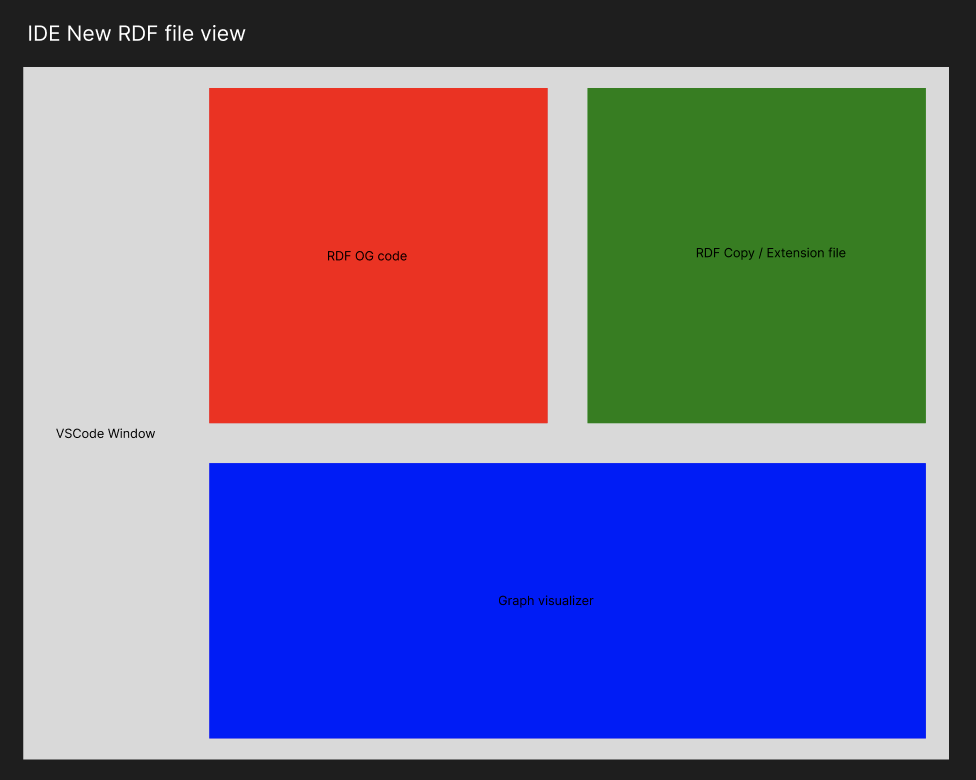
\includegraphics[width=14cm]{mock_ide_new_RDF_instance.png}\\
      \caption{IDE new RDF side panel view}\label{fig:IDERDFReader}
    \end{figure}

  \subsection{Server\label{sec:server}}
  To assure system intercompatibility across various device, Operative Systems, and User-Agents, the server is responsible for all computational tasks and data processing. By centralizing calculations and graph data manipulation on the server side, the server minimizes client-side resource consumption and enhances performance consistency. 
  \\
  \\
  The server place a crucial role in managing RDF data ensuring  schema validation, instance generation, SPARQL query processing, and graph construction.
  \\
  When the server receives an RDF file, it must scan the file to see potential floss, syntactic or semantic errors. It should be able to handle multiple RDF serialization formats such as Turtle, N3, XML, and JSON-LD. 
  \\
  \\
  The service generates synthetic RDF instances based on a given schema. It ensures logical consistency between the generated schema and the original one.
  \\
  The system identifies classes and properties within an RDF schema and generates additional instances, where necessary, to maintain semantic correctness. 
  \\
  This is particularly important in cases where a property references an instance of a specific class that has not been explicitly defined in the dataset.
  For example, if a schema includes a hasCar property that requires an instance of the Car class, but no such instance exists, the system should automatically create one. This ensures that the schema remains logically consistent and that all property constraints are met. By dynamically generating required instances, the system helps maintain data integrity, prevents incomplete assertions, and improves the reliability of reasoning processes within RDF applications.
  \\ 
  The additional generated instances have realistic properties and values in order to fulfill the graph constraints.
  \\
  \\
  The service serves the new RDF file in the requested format with its graphical representation.
    \chapter{Concept\label{cha:chapter4}}
This chapter introduces the architectural design of Component X. The component consists of subcomponent A, B and C.

In the end of this chapter you should write a specification for your solution, including interfaces, protocols and parameters.

\section{Sub-component A\label{sec:conceptsuba}}
The concept chapter provides a high-level explanation of your solution. Try to explain the overall structure with a picture. You can also use UML sequence diagrams for explanation.

Figure \ref{fig:aliceandbob} illustrates the situation between Alice and Bob. (sequence diagram from www.websequencediagrams.com)

\begin{figure}[htb]
  \centering
  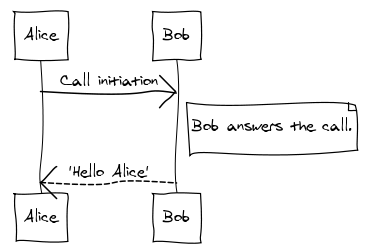
\includegraphics[width=9cm]{uml_seq_example.png}\\
  \caption{Alice and Bob}
  \label{fig:aliceandbob}
\end{figure}

\section{Sub-component B\label{sec:conceptsubb}}

Lorem Ipsum...

\section{Proposed API\label{sec:conceptapi}}

Lorem Ipsum...

\section{Layer X\label{sec:conceptlayerx}}

Lorem Ipsum...

\section{Interworking of X and Y\label{sec:conceptinter}}

Lorem Ipsum...

\section{Interface Specification\label{sec:intspec}}

Lorem Ipsum...


    \chapter{Evaluation\label{cha:chapter5}}

This chapter describes the evaluation method and results for the developed software solutions. 
The evaluation is divided into three main sections: 
\begin{itemize}
    \item Functional Evaluation
    \item Performance Evaluation
    \item Edge cases Analysis
\end{itemize}

All the test has been executed on the same machine, with the same configuration. \paragraph{Test Environment} Intel Core i7, 16 GB RAM, MacOS 15.4.1 

    

% Start 

\section{Functional Evaluation}

\subsection{Instance Generation}

\paragraph{Goal}
The first core functionality to evaluate is the \textbf{automatic generation of RDF instances}. This feature assist users by generating RDF instances based on a given RDF schema .

\paragraph{Test Description}
To validate this capability, two test scenarios were conducted:
\begin{itemize}
    \item \textbf{Test 1.1}: Generate instances from an RDF schema without additional properties.
    \item \textbf{Test 1.2}: Generate instances from an RDF schema and search for additional properties.
\end{itemize}

\subsubsection{Expected Result}

In the first case, the system was expected to:
\begin{itemize}
    \item Correctly generate RDF instances for each class.
    \item Ensure that instances respect domain and range restrictions.
    \item Keep the schema original schema structure intact, without any modifications in the classes or properties definitions.
\end{itemize}

In the second case, the system was expected to:
\begin{itemize}
    \item Correctly generate RDF instances for each class.
    \item Correctly generate additional properties for instance of non-implicitly referolive classes. 
    \item Ensure that instances respect domain and range restrictions.
    \item Keep the schema original schema structure intact, without any modifications in the classes or properties definitions.
\end{itemize}


\paragraph{Test Environment}
\begin{itemize}
    \item Test device: Intel Core i7, 16 GB RAM, MacOS 15.4.1 
\end{itemize}

\subsubsection{Actual Results}

The following two code sample, are the results of the two tests cases. For both the cases, the same RDF schema was provided. The code lines highlighted in olive green represent the synthetic instances generated by system. Three new instances were requested to be generated.
\\
Each of them has been marked as passed.
\\
\begin{lstlisting}[caption={Result Test Case 1.1}, label={lst:three-rdf-instances}]
    @prefix ex: <http://example.org/> .
    @prefix foaf: <http://xmlns.com/foaf/0.1/> .
    @prefix rdf: <http://www.w3.org/1999/02/22-rdf-syntax-ns#> .
    @prefix rdfs: <http://www.w3.org/2000/01/rdf-schema#> .
    @prefix schema1: <http://schema.org/> .
    @prefix xsd: <http://www.w3.org/2001/XMLSchema#> .
    
    ex:Employee a rdfs:Class ;
        rdfs:label "Employee" ;
        rdfs:comment "A class representing an employee." ;
        rdfs:subClassOf foaf:Person .
    
    (*@\textcolor{olive}{ex:Employee\_Instance1 a ex:Employee ;}@*)
        (*@\textcolor{olive}{ex:age 0 ;}@*)
        (*@\textcolor{olive}{ex:hasCar ex:Car\_Instance1 ;}@*)
        (*@\textcolor{olive}{ex:hasProfilePic ex:Image\_Instance1 ;}@*)
        (*@\textcolor{olive}{ex:isAtHome false ;}@*)
        (*@\textcolor{olive}{ex:ishuman "unknown"\textasciicircum{}\textasciicircum{}xsd:string .}@*)
    
    (*@\textcolor{olive}{ex:Employee\_Instance2 a ex:Employee ;}@*)
        (*@\textcolor{olive}{ex:age 0 ;}@*)
        (*@\textcolor{olive}{ex:hasCar ex:Car\_Instance2 ;}@*)
        (*@\textcolor{olive}{ex:hasProfilePic ex:Image\_Instance2 ;}@*)
        (*@\textcolor{olive}{ex:isAtHome false ;}@*)
        (*@\textcolor{olive}{ex:ishuman "unknown"\textasciicircum{}\textasciicircum{}xsd:string .}@*)
    
    (*@\textcolor{olive}{ex:Employee\_Instance3 a ex:Employee ;}@*)
        (*@\textcolor{olive}{ex:age 0 ;}@*)
        (*@\textcolor{olive}{ex:hasCar ex:Car\_Instance3 ;}@*)
        (*@\textcolor{olive}{ex:hasProfilePic ex:Image\_Instance3 ;}@*)
        (*@\textcolor{olive}{ex:isAtHome false ;}@*)
        (*@\textcolor{olive}{ex:ishuman "unknown"\textasciicircum{}\textasciicircum{}xsd:string .}@*)
    
    (*@\textcolor{olive}{ex:Person\_Instance1 a foaf:Person .}@*)
    
    (*@\textcolor{olive}{ex:Person\_Instance2 a foaf:Person .}@*)
    
    (*@\textcolor{olive}{ex:Person\_Instance3 a foaf:Person .}@*)
    
    ex:age a rdf:Property ;
        rdfs:domain ex:Employee ;
        rdfs:range xsd:integer .
    
    ex:hasCar a rdf:Property ;
        rdfs:label "hasCar" ;
        rdfs:comment "A property linking an employee to their car." ;
        rdfs:domain ex:Employee ;
        rdfs:range schema1:Car .
    
    ex:hasProfilePic a rdf:Property ;
        rdfs:domain ex:Employee ;
        rdfs:range foaf:Image .
    
    ex:isAtHome a rdf:Property ;
        rdfs:domain ex:Employee ;
        rdfs:range xsd:boolean .
    
    ex:ishuman a rdf:Property ;
        rdfs:domain ex:Employee ;
        rdfs:range xsd:string .
    
    (*@\textcolor{olive}{ex:Car\_Instance1 a schema1:Car .}@*)
    
    (*@\textcolor{olive}{ex:Car\_Instance2 a schema1:Car .}@*)
    
    (*@\textcolor{olive}{ex:Car\_Instance3 a schema1:Car .}@*)
    
    (*@\textcolor{olive}{ex:Image\_Instance1 a foaf:Image .}@*)
    
    (*@\textcolor{olive}{ex:Image\_Instance2 a foaf:Image .}@*)
    
    (*@\textcolor{olive}{ex:Image\_Instance3 a foaf:Image .}@*)
    \end{lstlisting}

    \begin{lstlisting}[caption={Result Test Case 1.2}, label={lst:three-rdf-instances-extended}]
@prefix ex: <http://example.org/> .
@prefix foaf: <http://xmlns.com/foaf/0.1/> .
@prefix rdf: <http://www.w3.org/1999/02/22-rdf-syntax-ns#> .
@prefix rdfs: <http://www.w3.org/2000/01/rdf-schema#> .
@prefix schema1: <http://schema.org/> .
@prefix xsd: <http://www.w3.org/2001/XMLSchema#> .

ex:Employee a rdfs:Class ;
    rdfs:label "Employee" ;
    rdfs:comment "A class representing an employee." ;
    rdfs:subClassOf foaf:Person .

(*@\textcolor{olive}{ex:Employee\_Instance1 a ex:Employee ;}@*)
    (*@\textcolor{olive}{ex:age 0 ;}@*)
    (*@\textcolor{olive}{ex:hasCar ex:Car\_Instance1 ;}@*)
    (*@\textcolor{olive}{ex:hasProfilePic ex:Image\_Instance1 ;}@*)
    (*@\textcolor{olive}{ex:isAtHome false ;}@*)
    (*@\textcolor{olive}{ex:ishuman "unknown"\textasciicircum{}\textasciicircum{}xsd:string .}@*)

(*@\textcolor{olive}{ex:Employee\_Instance2 a ex:Employee ;}@*)
    (*@\textcolor{olive}{ex:age 0 ;}@*)
    (*@\textcolor{olive}{ex:hasCar ex:Car\_Instance2 ;}@*)
    (*@\textcolor{olive}{ex:hasProfilePic ex:Image\_Instance2 ;}@*)
    (*@\textcolor{olive}{ex:isAtHome false ;}@*)
    (*@\textcolor{olive}{ex:ishuman "unknown"\textasciicircum{}\textasciicircum{}xsd:string .}@*)

(*@\textcolor{olive}{ex:Employee\_Instance3 a ex:Employee ;}@*)
    (*@\textcolor{olive}{ex:age 0 ;}@*)
    (*@\textcolor{olive}{ex:hasCar ex:Car\_Instance3 ;}@*)
    (*@\textcolor{olive}{ex:hasProfilePic ex:Image\_Instance3 ;}@*)
    (*@\textcolor{olive}{ex:isAtHome false ;}@*)
    (*@\textcolor{olive}{ex:ishuman "unknown"\textasciicircum{}\textasciicircum{}xsd:string .}@*)

(*@\textcolor{olive}{ex:Person\_Instance1 a foaf:Person ;}@*)
    (*@\textcolor{olive}{foaf:name "FedX" .}@*)

(*@\textcolor{olive}{ex:Person\_Instance2 a foaf:Person ;}@*)
    (*@\textcolor{olive}{foaf:name "FedX" .}@*)

(*@\textcolor{olive}{ex:Person\_Instance3 a foaf:Person ;}@*)
    (*@\textcolor{olive}{foaf:name "FedX" .}@*)

ex:age a rdf:Property ;
    rdfs:domain ex:Employee ;
    rdfs:range xsd:integer .

ex:hasCar a rdf:Property ;
    rdfs:label "hasCar" ;
    rdfs:comment "A property linking an employee to their car." ;
    rdfs:domain ex:Employee ;
    rdfs:range schema1:Car .

ex:hasProfilePic a rdf:Property ;
    rdfs:domain ex:Employee ;
    rdfs:range foaf:Image .

ex:isAtHome a rdf:Property ;
    rdfs:domain ex:Employee ;
    rdfs:range xsd:boolean .

ex:ishuman a rdf:Property ;
    rdfs:domain ex:Employee ;
    rdfs:range xsd:string .

(*@\textcolor{olive}{ex:Car\_Instance1 a schema1:Car ;}@*)
    (*@\textcolor{olive}{schema1:image ex:systems\_and\_procedures.svg\_Instance1 .}@*)

(*@\textcolor{olive}{ex:Car\_Instance2 a schema1:Car ;}@*)
    (*@\textcolor{olive}{schema1:image ex:systems\_and\_procedures.svg\_Instance2 .}@*)

(*@\textcolor{olive}{ex:Car\_Instance3 a schema1:Car ;}@*)
    (*@\textcolor{olive}{schema1:image ex:systems\_and\_procedures.svg\_Instance3 .}@*)

(*@\textcolor{olive}{ex:Image\_Instance1 a foaf:Image ;}@*)
    (*@\textcolor{olive}{foaf:name "Noel Ignatiev" .}@*)

(*@\textcolor{olive}{ex:Image\_Instance2 a foaf:Image ;}@*)
    (*@\textcolor{olive}{foaf:name "Noel Ignatiev" .}@*)

(*@\textcolor{olive}{ex:Image\_Instance3 a foaf:Image ;}@*)
    (*@\textcolor{olive}{foaf:name "Noel Ignatiev" .}@*)

(*@\textcolor{olive}{ex:systems\_and\_procedures.svg\_Instance1 a <https://raw.githubusercontent.com/OpenHPS/POSO/main/docs/images/systems\_and\_procedures.svg> .}@*)

(*@\textcolor{olive}{ex:systems\_and\_procedures.svg\_Instance2 a <https://raw.githubusercontent.com/OpenHPS/POSO/main/docs/images/systems\_and\_procedures.svg> .}@*)

(*@\textcolor{olive}{ex:systems\_and\_procedures.svg\_Instance3 a <https://raw.githubusercontent.com/OpenHPS/POSO/main/docs/images/systems\_and\_procedures.svg> .}@*)
\end{lstlisting}

\paragraph{Comments}
The simple instance generation was handled smoothly, completing instance generation in under 1 second.  
In the instance generation with property search case, although generation succeeded, a delay of approximately 40 seconds was observed during the function execution.
This is due to the time required to search for additional properties in the Linked Open Vocabularies system.  
No critical issues were found. 
\\
Future work could include optimization of generation and property search algorithm, maybe with the use of multithreading and parallel processing.

% End 

% Start 
\subsection{Graph visualization}

\paragraph{Goal}
The second-biggest functionality to evaluate is the \textbf{Graph visualization}. This feature allow user to better see the instances that have been generated thanks to their graph representation.

\paragraph{Test Description}
To validate this capability, the following test scenarios were conducted:
\begin{itemize}
    \item \textbf{Test 2.1}: After the server response, a graph visualization is generated in the provided canvas - on Browser. 
    \item \textbf{Test 2.2}: After the server response, a graph visualization is generated in the provided canvas - on VSCode. 
\end{itemize}

\subsubsection{Expected Result}

In the both the scenarios, the expected results are:
\begin{itemize}
    \item Correctly visualize the canvas with the related graph.
    \item Be able to interact with the graph (i.e. clicking and highlighting nodes, move nodes, zooming in and out).
\end{itemize}

\subsubsection{Actual Results}

The following image, is an example resutl of the tests cases.
\\
Each of them has been marked as passed.
\\

\begin{figure}[htb]
    \centering
    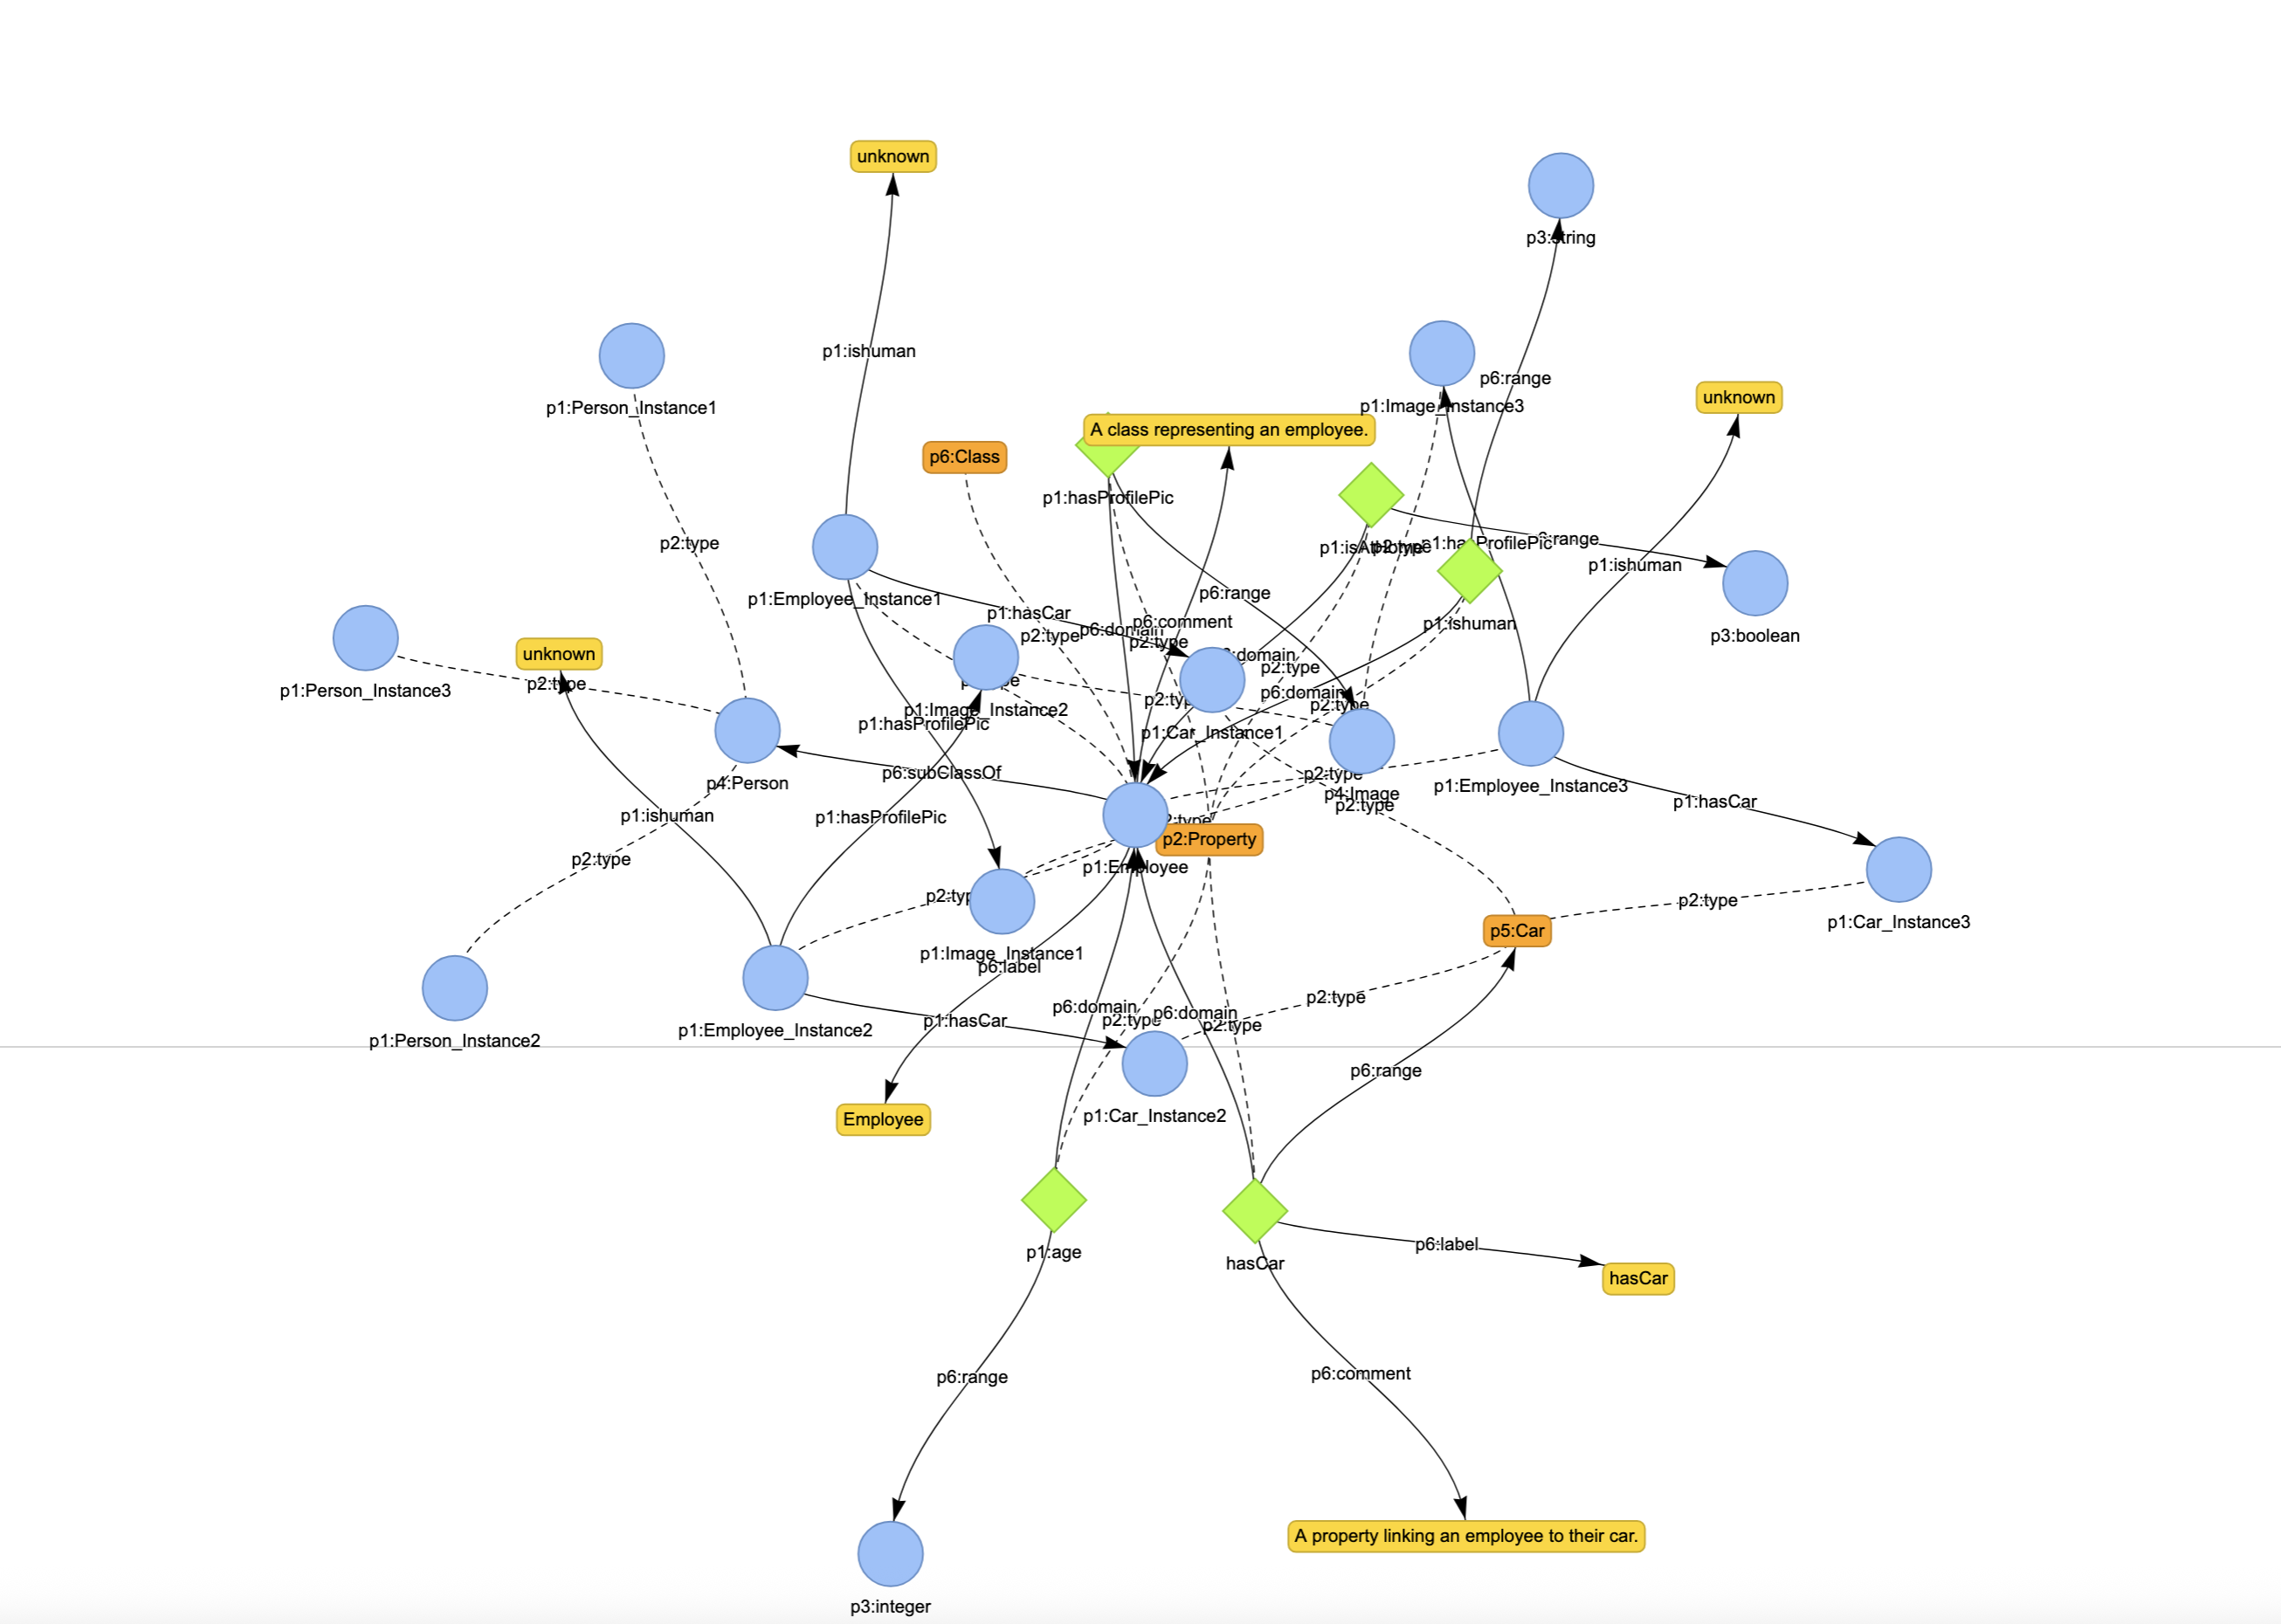
\includegraphics[width=14cm]{graphviewbrowserevaluation.png}
    \caption{Rending of the RDF graph}
    \label{fig:rendergraph}
\end{figure}

\paragraph{Comments}
For both the scenarios the graphs have been rendered correctly and no critical issues were found.
Unfortunately, I could find a way to stabilize the graph rendering in order to have the very same in the same place at each render. This would have help the user to better visualize the graph in case of some live edits in the RDF schema. 
\\
Some future work could include a better rendering engine and node distribution on the canvas.
% End 

% Start 
\subsection{RDF Graph and Schema Export}

\paragraph{Goal}
The next capability to evaluate is the \textbf{RDF Graph and Schema Export}. The user must be able to export the RDF schema and the generated graph.

\paragraph{Test Description}
To validate this functions, the following test scenarios were conducted:
\begin{itemize}
    \item \textbf{Test 3.1}: After the server response, a button allows to download the newly generated RDF schema - on Browser. 
    \item \textbf{Test 3.2}: After the server response, a button allows to visualize the newly generated schema in a new IDE window - on VSCode. 
    \item \textbf{Test 3.3}: After the server response, a button allows to export the RDF graph in a png format - on Browser. 
    \item \textbf{Test 3.4}: After the server response, a button allows to export the RDF graph in a png format - on VSCode. 
\end{itemize}

\subsubsection{Expected Result}

For two initial tests (\textbf{Test 3.1} and \textbf{Test 3.2}) scenario, the expected results are:
\begin{itemize}
    \item The correct generation of the download button.
    \item No anomalies in the download file. 
\end{itemize}

The remaining two tests (\textbf{Test 3.3} and \textbf{Test 3.4}), are expected to:
\begin{itemize}
    \item Generate a button that allow the graph to be exported in a PNG format. 
    \item The image graph in the PNG file is consistent with the one visualized in the application canvas.
\end{itemize}

\subsubsection{Actual Results}

The figure \ref{fig:schemadownload} showcase the first two test cases. The performed action has been marked with a red circle.
The outcome of the action is marked in a light green square. 

The figure \ref{fig:graphdownloadfrombrowsersandIDE} is the result of the last two test cases. The same marking process has also been in use in this figure.

All of them has been marked as passed.
\\

\begin{figure}[htb]
    \centering
    \begin{subfigure}[b]{0.48\textwidth}
        \centering
        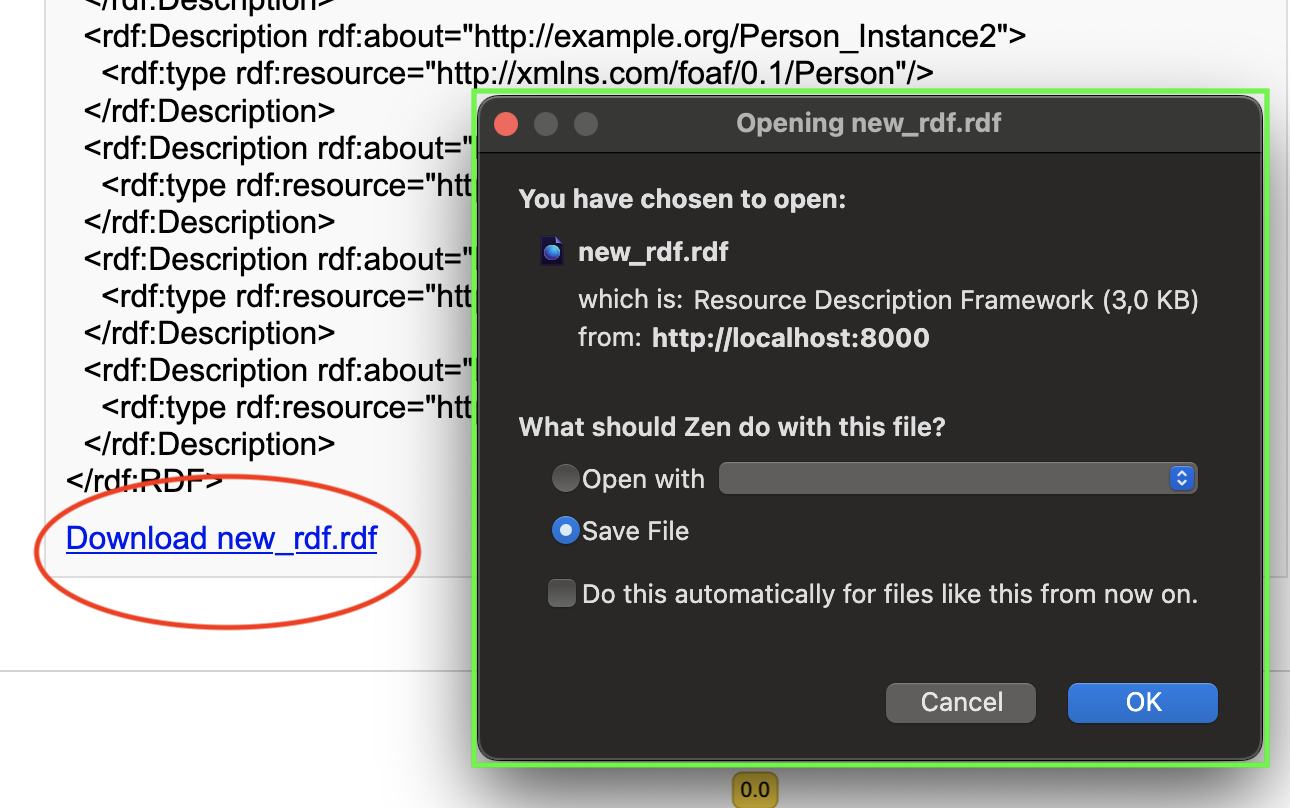
\includegraphics[width=\textwidth]{schemadownloadBrowser.png}
        \caption{Click action on the download button to download the RDF schema}
        \label{fig:RDFschemadownloadA}
    \end{subfigure}
    \hfill
    \begin{subfigure}[b]{0.48\textwidth}
        \centering
        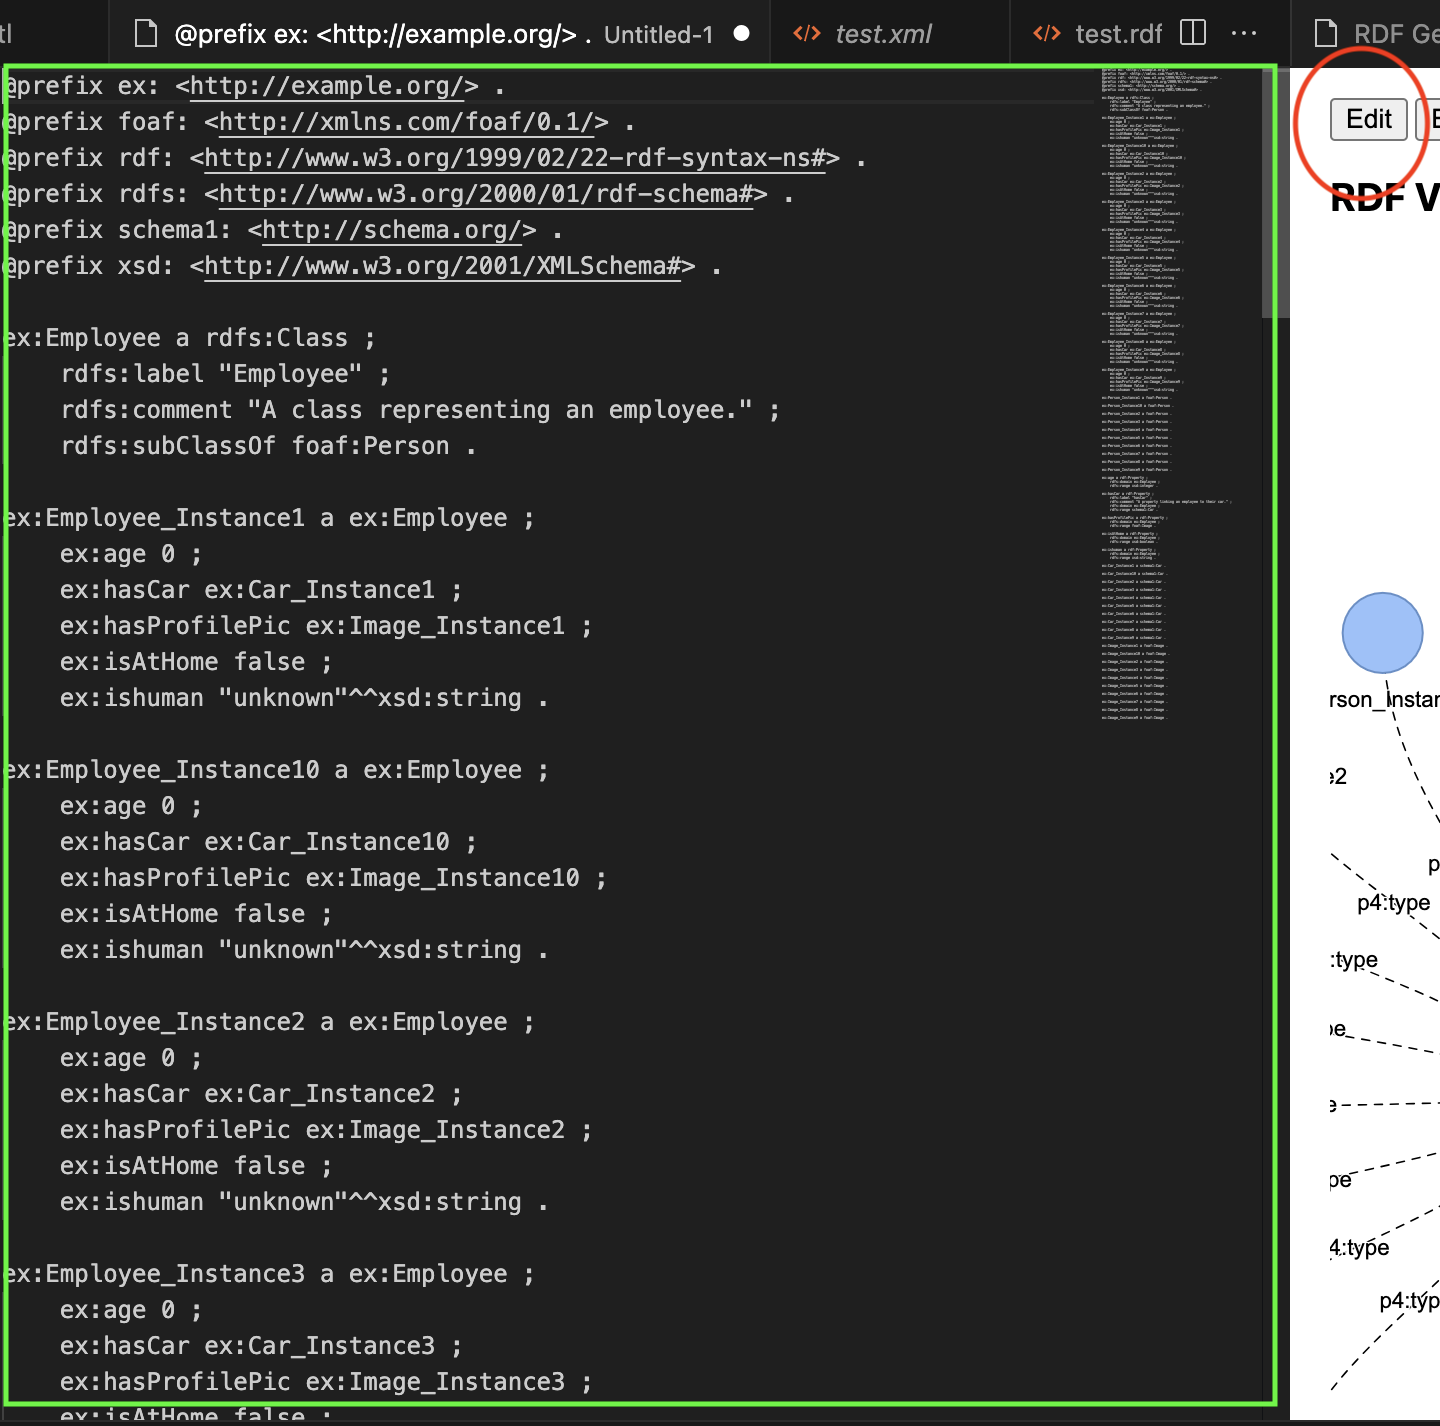
\includegraphics[width=\textwidth]{schemadownloadIDE.png}
        \caption{Click action on the edit button to download/edit the RDF schema}
        \label{fig:RDFschemadownloadB}
    \end{subfigure}
    \caption{RDF Schema download methods for Browsers client and IDE client}
    \label{fig:schemadownload}
\end{figure}

\begin{figure}[H]
    \centering
    \begin{subfigure}[b]{0.48\textwidth}
        \centering
        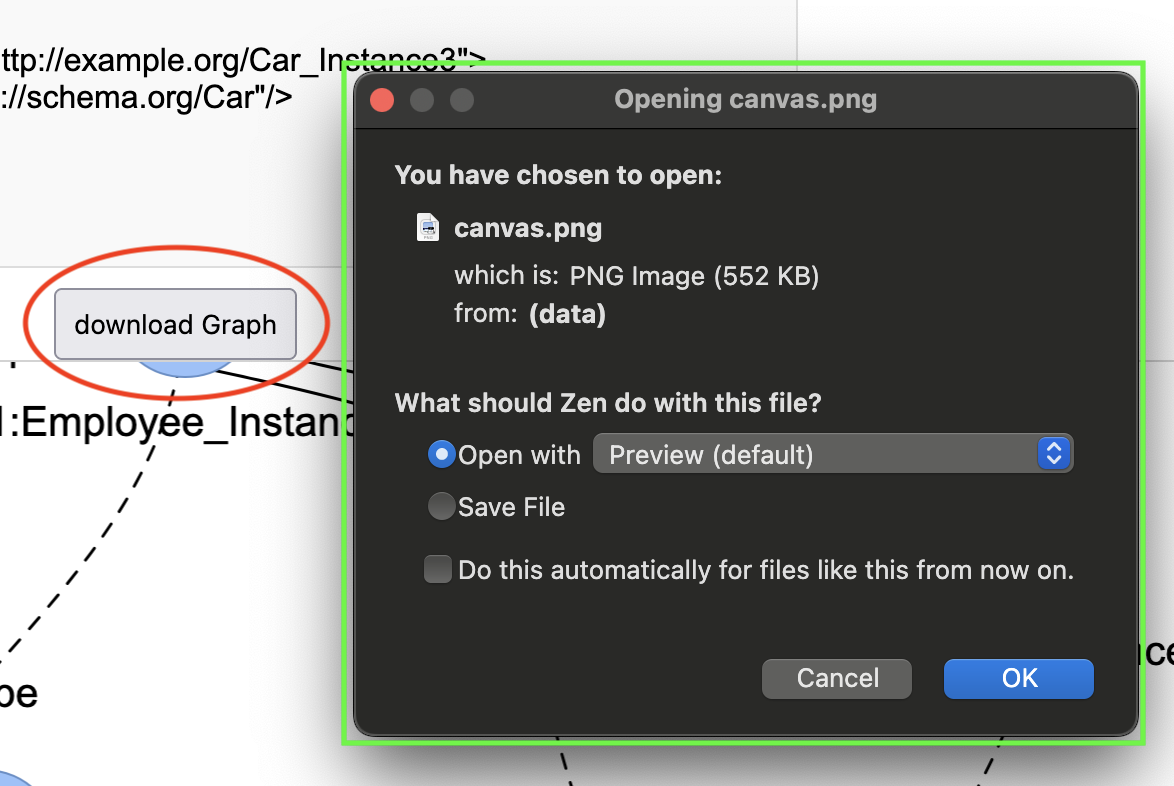
\includegraphics[width=\textwidth]{graphdownloadBrowser.png}
        \caption{Click action on the download button to download the RDF Graph}
        \label{fig:graphdownloadA}
    \end{subfigure}
    \hfill
    \begin{subfigure}[b]{0.48\textwidth}
        \centering
        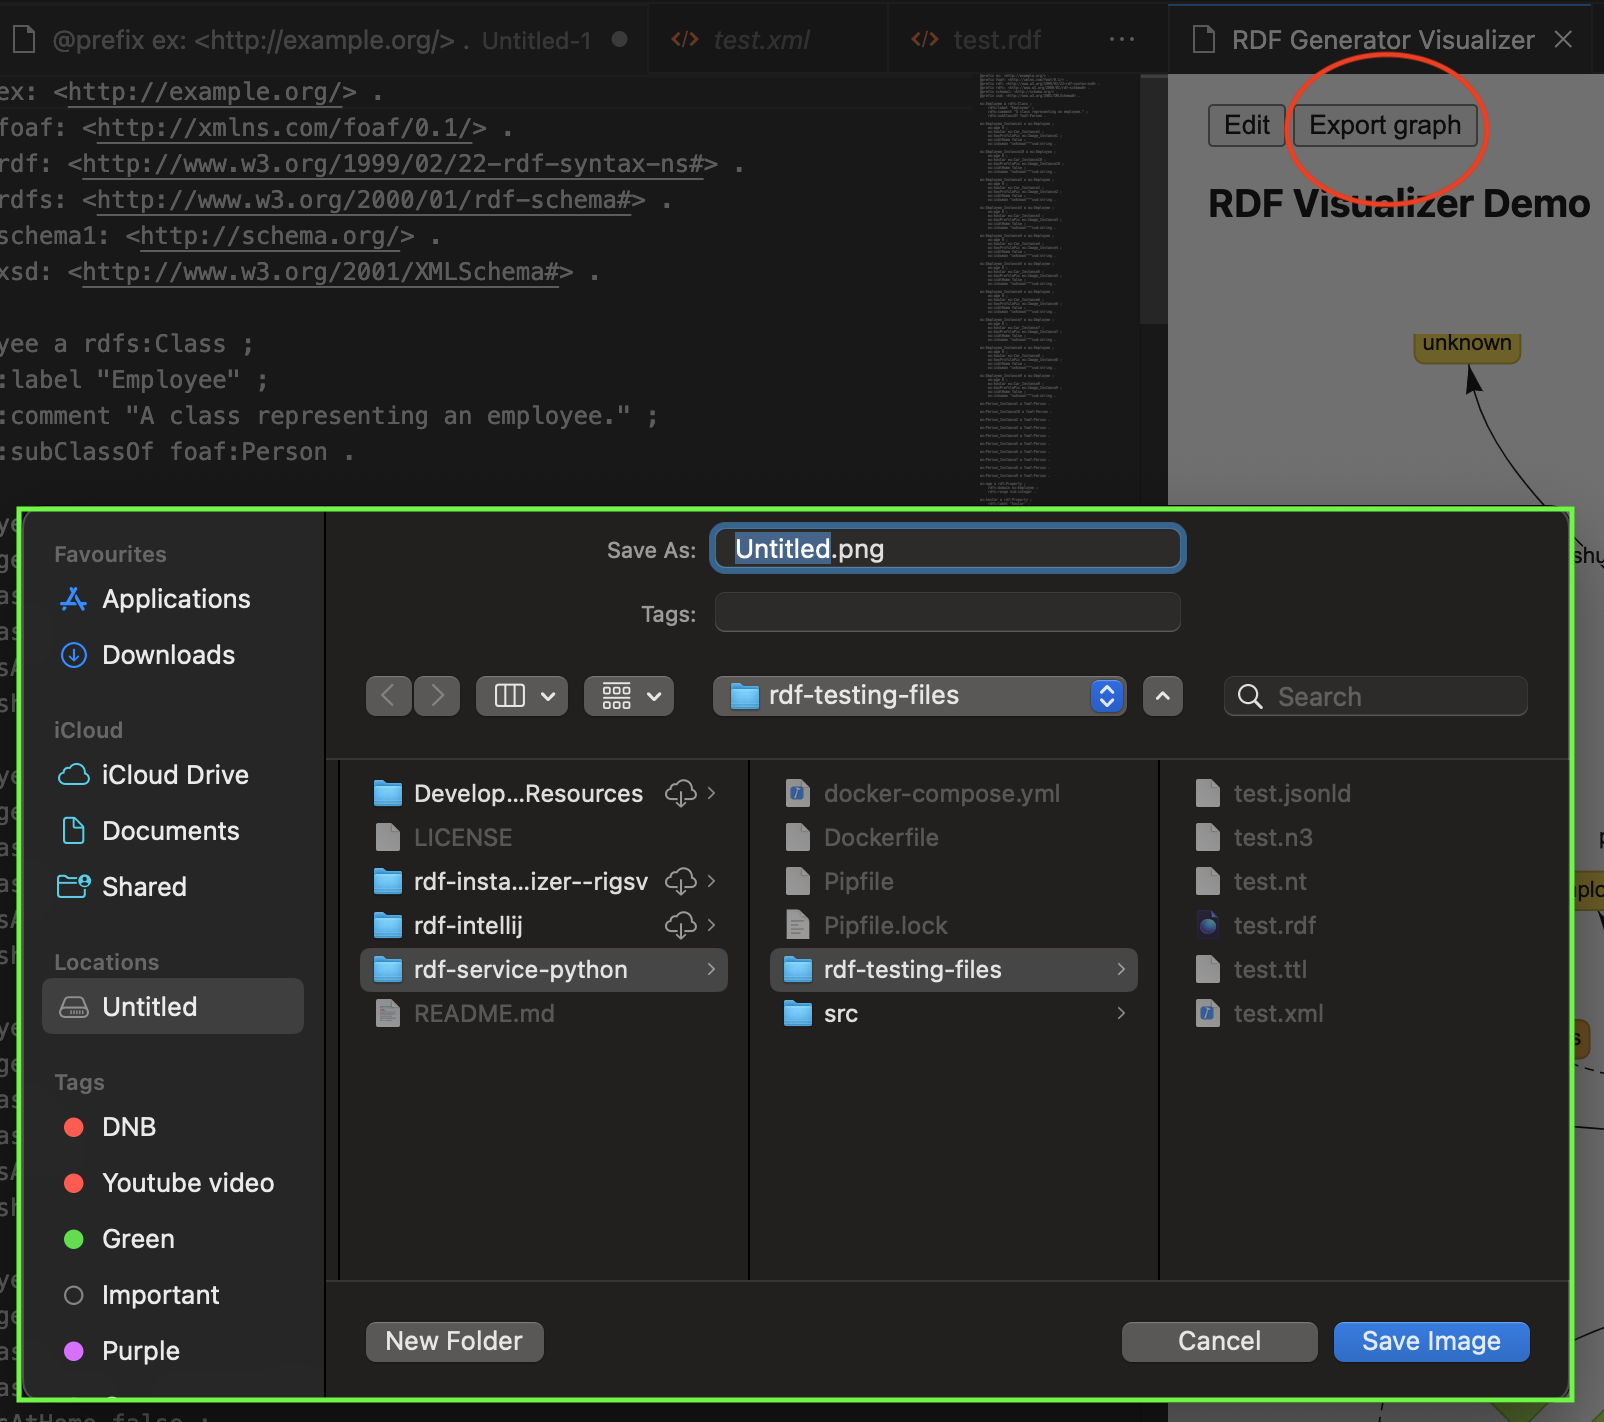
\includegraphics[width=\textwidth]{graphdownloadIDE.png}
        \caption{Rendering of RDF graph B}
        \label{fig:graphdownloadB}
    \end{subfigure}
    \caption{RClick action on the download button to download the RDF Graph}
    \label{fig:graphdownloadfrombrowsersandIDE}
\end{figure}


\paragraph{Comments}
All the test have passed and not critical issue were found the testing process.
Although one minore but has been found while testig the edit button in the IDE enviroment. 
\\
When the button is clicked and the schema is visualized in a new VSCode tab, if the user edits the file, it cannot be sent to the server directly. 
The file must be first saved and then sent to the server. Any action performed on a not saved file will cause the server to answer with an error. 

Future updated will provide a solution to the described bug and improvements in the RDF scheme edit mode, like allowing edits in the browser mode before the download and the options to re-render the graph automatically after a change in the file. 
% End 

\section{Performance Evaluation}
% Start Performance 1 
\subsection{Rendering Time}

\paragraph{Goal}
This test evaluates the responsiveness of the RDF visualization system by measuring the time required to render RDF graphs of increasing complexity. The rendering time is defined as the duration from server response to the completion of layout and DOM paint on canvas.

\paragraph{Method}
To test the rendering performance, three different schema sizes were generated:
\begin{itemize}
    \item \textbf{Small schema}: 10 instances generated
    \item \textbf{Medium schema}: 50 instances generated
    \item \textbf{Large schema}: 100 instances generated
\end{itemize}

Each rendering test was executed 3 times, and the average rendering time was recorded using \texttt{performance.now()} browser function.

\subsubsection{Results}

\begin{table}[H]
\centering
\begin{tabular}{|c|c|c|}
\hline
\textbf{Schema Size} & \textbf{Instances} & \textbf{Avg. Render Time (ms)} \\ \hline
Small & 10 & 121 \\ \hline
Medium & 50 & 4638 \\ \hline
Large & 100 & 9871 \\ \hline
\end{tabular}
\caption{Rendering time of RDF graphs with increasing complexity}
\label{tab:rendering-times}
\end{table}

\paragraph{Comments}
The results demonstrate a steep increase in rendering time with the number of nodes. While the small schema rendered almost instantly (121 ms), the medium and large schemas took 4.6 and 9.8 seconds respectively. This nonlinear growth in rendering time is attributed to the physics-based layout engine used by vis.js.

The delays observed in medium and large graphs can negatively affect user experience. To guarantee a nice UX the instances that can be generated are limited to a maximum number of ten. Future optimizations could include:
\begin{itemize}
    \item Reducing the number of stabilization iterations for larger graphs.
    \item Using simplified layouts (e.g., hierarchical layout).
    \item Introducing progressive or chunked rendering for large datasets.
\end{itemize}


\subsection{Instance generation time}

\paragraph{Goal}
This test evaluates the responsiveness of the RDF instance generation system (with no properties search) from the incoming request to the server response.

\paragraph{Method}
To test the rendering performance, three different schema sizes were generated:
\begin{itemize}
    \item \textbf{Small schema}: 10 instances generated
    \item \textbf{Medium schema}: 50 instances generated
    \item \textbf{Large schema}: 100 instances generated
\end{itemize}

Each generation test was executed 3 times, and the average response time was recorded using the \texttt{Time} python library.

\subsubsection{Results}

\begin{table}[H]
\centering
\begin{tabular}{|c|c|c|}
\hline
\textbf{Schema Size} & \textbf{Instances} & \textbf{Avg. Render Time (ms)} \\ \hline
Small & 10 & 36.2 \\ \hline
Medium & 50 & 98.0 \\ \hline
Large & 100 & 142.22 \\ \hline
\end{tabular}
\caption{Response time of RDF instance generator function with increasing complexity}
\label{tab:rendering-times}
\end{table}

\paragraph{Comments}
The results indicate that the instance generation time increases moderately with the number of instances requested. The small schema completed generation in approximately 36 ms, while the medium and large schemas required 98 ms and 142 ms respectively. Although the growth is not exponential, the system's responsiveness could degrade if the quality of the hardware is lowered.

To ensure a consistently smooth user experience, be coherent with the current graph visualization limit and avoid potential performance bottlenecks for machine with a low budget hardware, the current implementation limits instance generation to a maximum of ten instances per request. 

Future enhancements may explore asynchronous processing, or batched generation to support larger requests without compromising server responsiveness.
\\
\\
\subsection{Instance generation time with property search}

\paragraph{Goal}
This test evaluates the responsiveness of the RDF instance generation system, with properties search, from the incoming request to the server response.

\paragraph{Method}
To test the rendering performance, three different schema sizes were generated:
\begin{itemize}
    \item \textbf{Small schema}: 1 instances generated
    \item \textbf{Medium schema}: 5 instances generated
    \item \textbf{Large schema}: 10 instances generated
\end{itemize}

Each generation test was executed one time only to not stress the LOV api service with testing request, and the average response time was recorded using the \texttt{Time} python library.

\subsubsection{Results}

\begin{table}[H]
\centering
\begin{tabular}{|c|c|c|}
\hline
\textbf{Schema Size} & \textbf{Instances} & \textbf{Avg. Render Time (ms)} \\ \hline
Small & 1 & 206592 \\ \hline
Medium & 5 & 215507\\ \hline
Large & 10 & 245350 \\ \hline
\end{tabular}
\caption{Response time of RDF instance generator function with propertiesn search}
\label{tab:rendering-times}
\end{table}

\paragraph{Comments}
The results reveal a surprising insight: the number of instances requested had minimal influence on the overall generation time. Instead, the dominant factor affecting performance was the number of properties that required semantic enrichment with the vocabulary lookup, specifically those whose ranges point to other classes.

This is explained by the fact that, for each such property, the system performs a query against the Linked Open Vocabularies (LOV) API to search for semantically relevant property names. As the number of properties requiring lookup increases, so does the total response time, regardless of the number of instances being generated.

Due to this dependency on an external service and its associated latency, the current implementation limits instance generation with property search to a maximum of 3 instances with only 1 property enhancements per class. This helps reduce the number of API calls and ensures acceptable response times. 

Future improvements may include result caching, local vocabulary indexing and batching to enhance performance. 

% edge cases analysis
\subsection{Edge Case Analysis}

\paragraph{Goal}
This section evaluates how the system handles unexpected input scenarios that may occur during RDF instance generation. The objective is to ensure robustness and graceful failure handling, even when inputs deviate from normal expectations.

\paragraph{Method}
A series of edge case tests were conducted to assess the stability and correctness of the system in the following situations:

\begin{itemize}
    \item \textbf{Invalid file:} The input file is not an rdf file
    \item \textbf{Empty Schema:} Schema with no classes or properties defined.
    \item \textbf{Circular Class References:} A Class (A) has a property pointing to another Class (B), which points back to the previous Class.
    \item \textbf{Unsupported RDF Constructs:} Use of blank nodes or advanced RDF syntax that has not specifically handled.
    \item \textbf{Highly Connected Schema:} A class with more than 20 properties linking to multiple other classes.
    \item \textbf{Malformed Input:} Invalid RDF syntax.
\end{itemize}

Each scenario was executed through the instance generator and monitored for application stability, error messages, and correctness of the output.

\paragraph{Results}
The application performed robustly in most edge case scenarios. Table~\ref{tab:edge-case-results} summarizes the outcomes.

\begin{table}[H]
\centering
\begin{tabular}{|p{4.5cm}|p{3cm}|p{6cm}|}
\hline

\textbf{Test Case} & \textbf{Status} & \textbf{Notes} \\ \hline 
Invalid file & Partial & Server returned a generic error response (\textit{Error loading content}). \\ \hline
Empty Schema & Pass & Server returned an empty canvas with no errors. \\ \hline
Circular Class References & Pass & Instance generation completed; circular references were handled without infinite loops. \\ \hline
Unsupported RDF Constructs & Pass & Blank nodes were handled without failure; no warning issued. \\ \hline
Highly Connected Schema & Partial & Significant performance degradation observed in the rendering of the graph. \\ \hline
Malformed Input & Partial & Server returned a generic error response (\textit{Error loading content}). \\ \hline
\end{tabular}
\caption{Summary of edge case testing outcomes}
\label{tab:edge-case-results}
\end{table}

\paragraph{Comments}
The system demonstrates strong resilience against most edge cases. In particular, circular class references and highly nested schemas did not lead to crashes or infinite loops. However, two weak points were identified: the invalid file and malformed input.
Addressing these cases would improve user experience and system robustness.
    \chapter{Evaluation\label{cha:chapter6}}

In this chapter the implementation of Component X is evaluated. An example instance was created for every service. The following chapter validates the component implemented in the previous chapter against the requirements.
\\
\\
Put some screenshots in this section! Map the requirements with your proposed solution. Compare it with related work. Why is your solution better than a concurrent approach from another organization?

\section{Test Environment\label{sec:testenvir}}

Fraunhofer Institute FOKUS' Open IMS Playground was used as a test environment for the telecommunication services. The IMS Playground ...

\section{Scalability\label{sec:scal}}

Lorem Ipsum

\section{Usability\label{sec:usab}}

Lorem Ipsum

\section{Performance Measurements\label{sec:performance}}

Lorem Ipsum
    \chapter{Outlook\label{cha:chapter7}}
The final chapter summarizes the thesis. The first subsection outlines the main ideas behind Component X and recapitulates the work steps. Issues that remained unsolved are then described. Finally the potential of the proposed solution and future work is surveyed in an outlook.

\section{Summary\label{sec:summary}}

Explain what you did during the last 6 month on 1 or 2 pages!
\\
\\
\noindent The work done can be summarized into the following work steps

\begin{itemize}
		\item Analysis of available technologies
		\vspace{-0.11in} 
		\item Selection of 3 relevant services for implementation
		\vspace{-0.11in} 
		\item Design and implementation of X on Windows
		\vspace{-0.11in} 
		\item Design and implementation of X on mobile devices
		\vspace{-0.11in} 
		\item Documentation based on X
		\vspace{-0.11in} 
		\item Evaluation of the proposed solution
\end{itemize}

\section{Dissemination\label{sec:dissemination}}

Who uses your component or who will use it? Industry projects, EU projects, open source...? Is it integrated into a larger environment? Did you publish any papers?

\section{Problems Encountered\label{sec:problems}}

Summarize the main problems. How did you solve them? Why didn't you solve them?

\section{Outlook\label{sec:outlook}}

Future work will enhance Component X with new services and features that can be used ...

% ---------------------------------------------------------------
\backmatter % no page numbering from here
    \todo[inline]{talk to your supervisor if this is needed}
    \addchap{List of Acronyms}

\begin{tabbing}
spacespacespace \= space \kill
3GPP	 \> 	3rd Generation Partnership Project	 \\
AJAX	\>	Asynchronous JavaScript and XML \\
API	 \> 	Application Programming Interface	 \\
AS	\>	Application Server \\
CSCF	 \> 	Call Session Control Function	 \\
CSS	\>	Cascading Stylesheets \\
DHTML	\>	Dynamic HTML \\
DOM	\>	Document Object Model \\
FOKUS	\>	Fraunhofer Institut fuer offene Kommunikationssysteme \\
GUI	\>	Graphical User Interface \\
GPS	\>	Global Positioning System \\
GSM	\>	Global System for Mobile Communication\\
HTML	\>	Hypertext Markup Language \\
HSS	 \> 	Home Subscriber Server	 \\
HTTP	 \> 	Hypertext Transfer Protocol	 \\
I-CSCF	 \> 	Interrogating-Call Session Control Function	 \\
IETF	\>	Internet Engineering Task Force \\
IM	\>	Instant Messaging \\
IMS	 \> 	IP Multimedia Subsystem	 \\
IP	 \> 	Internet Protocol	 \\
J2ME	\>	Java Micro Edition \\
JDK	\>	Java Developer Kit \\
JRE	\>	Java Runtime Environment \\
JSON	\>	JavaScript Object Notation \\
JSR	\>	Java Specification Request \\
JVM	 \> 	Java Virtual Machine	 \\
NGN	 \> 	Next Generation Network	 \\
OMA	 \> 	Open Mobile Alliance	 \\
P-CSCF	 \> 	Proxy-Call Session Control Function	 \\
PDA	\>	Personal Digital Assistant \\
PEEM	 \> 	Policy Evaluation, Enforcement and Management	 \\
QoS	 \> 	Quality of Service	 \\
S-CSCF	 \> 	Serving-Call Session Control Function	 \\
SDK	\>	Software Developer Kit \\
SDP	\>	Session Description Protocol \\
SIP	 \> 	Session Initiation Protocol	 \\
SMS	\>	Short Message Service \\
SMSC	\> Short Message Service Center \\
SOAP	 \> 	Simple Object Access Protocol	 \\
SWF	\>	Shockwave Flash \\
SWT	\>	Standard Widget Toolkit \\
TCP	 \> 	Transmission Control Protocol	 \\
Telco API	\>	Telecommunication API \\
TLS	\>	Transport Layer Security \\
UMTS	 \> 	Universal Mobile Telecommunication System	 \\
URI	 \> 	Uniform Resource Identifier	 \\
VoIP	 \> 	Voice over Internet Protocol	 \\
W3C	 \> 	World Wide Web Consortium	 \\
WSDL	\>	Web Service Description Language \\
XCAP	 \> 	XML Configuration Access Protocol	 \\
XDMS	 \> 	XML Document Management Server	 \\
XML	 \> 	Extensible Markup Language	 \\
\end{tabbing}
\endinput

		
		% if you want to provide a glossary with explanations of important terms put it in here

    \bibliographystyle{geralpha}
    \bibliography{./bib/manual}
    
    \addchap{Annex}

\begin{appendix}

\lstset{language=,caption=Sourcecode Listing,captionpos=b,
label=yahoowidgetkon,showstringspaces=false,
basicstyle={\fontfamily{pcr}\selectfont\footnotesize}}
\begin{lstlisting}
<?xml version="1.0" encoding="UTF-8"?>
<widget>
	 <debug>off</debug>
	 <window name="myWindow" title="Hello Widget" visible="true">
		 <height>120</height>
		 <width>320</width>
		 <image src="Resources/orangebg.png">
			<name>orangebg</name>
			<hOffset>0</hOffset>
			<vOffset>0</vOffset>
		</image>
		 <text>
			 <name>myText</name>
			 <data>Hello Widget</data>
			 <color>#000000</color>
			 <size>20</size>
			 <vOffset>50</vOffset>
			 <hOffset>120</hOffset>
		 </text>
	</window>
</widget>
\end{lstlisting}

\newpage


\lstset{caption=SIP request and response packet\cite{SIPBook},
captionpos=b,label=sippacket,showstringspaces=false,
basicstyle={\fontfamily{pcr}\selectfont\footnotesize}}
\begin{lstlisting}
INVITE sip:bob@network.org SIP/2.0
Via: SIP/2.0/UDP 100.101.102.103:5060;branch=z9hG4bKmp17a
Max-Forwards: 70
To: Bob <sip:bob@network.org>
From: Alice <sip:alice@ims-network.org>;tag=42
Call-ID: 10@100.101.102.103
CSeq: 1 INVITE
Subject: How are you?
Contact: <sip:xyz@network.org>
Content-Type: application/sdp
Content-Length: 159
v=0
o=alice 2890844526 2890844526 IN IP4 100.101.102.103
s=Phone Call
t=0 0
c=IN IP4 100.101.102.103
m=audio 49170 RTP/AVP 0
a=rtpmap:0 PCMU/8000

SIP/2.0 200 OK
Via: SIP/2.0/UDP proxy.network.org:5060;branch=z9hG4bK83842.1
;received=100.101.102.105
Via: SIP/2.0/UDP 100.101.102.103:5060;branch=z9hG4bKmp17a
To: Bob <sip:bob@network.org>;tag=314159
From: Alice <sip:alice@network.org>;tag=42
Call-ID: 10@100.101.102.103
CSeq: 1 INVITE
Contact: <sip:foo@network.org>
Content-Type: application/sdp
Content-Length: 159
v=0
o=bob 2890844526 2890844526 IN IP4 200.201.202.203
s=Phone Call
c=IN IP4 200.201.202.203
t=0 0
m=audio 49172 RTP/AVP 0
a=rtpmap:0 PCMU/8000
\end{lstlisting}


\end{appendix}

\endinput


\end{document}
